\documentclass{article}

% Language setting Replace `english' with e.g. `spanish' to change the document
% language
\usepackage[english]{babel}
\usepackage{caption}
\usepackage{subcaption}
\usepackage{makecell}
\usepackage[toc,page]{appendix}
\setlength{\marginparwidth}{2cm}
\usepackage{todonotes}
\usepackage{soul}
\usepackage{pdflscape}


% Set page size and margins Replace `letterpaper' with `a4paper' for UK/EU
% standard size
\usepackage[letterpaper,top=2cm,bottom=2cm,left=3cm,right=3cm,marginparwidth=1.75cm]{geometry}

% Useful packages
\usepackage{amsmath}
\usepackage{amsfonts}
\usepackage{amssymb}
\usepackage{graphicx}
\usepackage{xspace}
\usepackage{xcolor}% http://ctan.org/pkg/xcolor
\usepackage{hyperref}
\usepackage{colortbl}
\usepackage{dsfont}

\setlength{\marginparwidth}{2cm}
\usepackage{todonotes}

\newcommand{\TODO}[1]{\color{red}\textsc{TODO:} #1\color{black}\xspace}
\newcommand{\TG}[1]{\color{blue}\textsc{From Tristan:} #1\color{black}\xspace}
\newcommand{\fmriprep}{fMRIPrep \xspace}
\newcommand{\fwhm}{\textsc{FWHM}}

\newcommand\Mark[2][8.4]{%
  \rlap{\tikz[baseline=(current bounding box.south)]{
        \shade[left color=\color{red}, right color=\color{green}, middle color=\color{yellow}]
               (0,0) rectangle ++(#1*#2/100,0.3);}%
  }%
}

% Cluster failure: Why fMRI inferences for spatial extent have inflated
% false-positive https://www.pnas.org/doi/pdf/10.1073/pnas.1602413113                       

\title{Non-regression tests for structural MRI analysis: towards a numerical uncertainty approach}
\author{Yohan Chatelain, Loic Tetrel, Christopher J. Markiewicz, Gregory Kiar,\\ Oscar Esteban,  Pierre Bellec, Tristan Glatard}

\begin{document}
\maketitle

\begin{abstract}
    Target: PLOS ONE, Frontiers in Neuroinformatics,  IEEE Transactions on
    Software Engineering. \url{https://www.computer.org/csdl/journal/ts}
\end{abstract}

\section{Introduction}

The need for and requirements of long-term support of neuroimaging software:
\begin{itemize}
    \item Span over several years. Software updates are unavoidable (security
          updates, EOL, etc).
    \item Neuroimaging software can be unstable, variation across packages are
          significant -> therefore need to be tested
    \item for instance: fmriprep LTS project
\end{itemize}

Non-regression testing in neuroimaging:
\begin{itemize}
    \item Testing is difficult because (1) there is no reference (ground truth),
          (2) as in many other contexts, defining an acceptable tolerance (variation
          bounds) is difficult.
    \item there are methods to evaluate software in the absence of ground truth
          (simulation, phantoms, ex-vivo) but they all have their own limitations and
          they don't allow for the definition of acceptable variation bounds.
    \item There are no widely accepted bounds of variation around any reference.
          Variation bounds may be defined specifically for each application (e.g.,
          from the measured effect on the F1 score of a classifier), but the stability
          of pre-processing must be guaranteed independently of any particular
          application.
    \item Our approach is to define a reference result and acceptable variation
          bounds around this reference from the numerical uncertainty measured in the
          reference software version. Using a set of representative datasets.
    \item Numerical variability is a critical property of scientific data
          analyses [ref Greg]. Numerical uncertainty may capture the variation that
          would be experienced by users when using the software tool in different
          environments including different hardware architectures and software stacks.
    \item We build on previous evaluations of numerical variability in
          neuroimaging: ref greg \& ali
    \item We measure this uncertainty using random rounding (references,
          summarize principle).
\end{itemize}

\begin{figure}

\end{figure}

The same method could be applied to other domains where ground truth is not
available or acceptable variation bounds cannot be easily defined.

Mention that based on previous results, libmath explains a large amount of
numerical variability observed across OS differences. Explain GNU libmath.

Define LTS as an arbitrary reference version of fMRIPrep.

Correcting for multiple comparisons is a challenge. Refer to main methods used
in neuroimaging. Explain that we have images, voxels, etc

fMRIPrep is a functional magnetic resonance imaging (fMRI) data preprocessing
pipeline designed to provide an easily accessible, state-of-the-art interface
that is robust to variations in scan acquisition protocols and that requires
minimal user input, while providing easily interpretable and comprehensive error
and output reporting. It performs basic processing steps (coregistration,
normalization, unwarping, noise component extraction, segmentation,
skullstripping etc.) to provide outputs that can be easily submitted to a
variety of group level analyses, including task-based or resting-state fMRI,
graph theory measures, surface or volume-based statistics, etc. We focused our
study on the structural analysis pipeline of fMRIPrep for simplicity.




Paper goal:
\begin{itemize}
    %\item G1: To measure the numerical variability of MRI structural analysis
    \item G1: Build and evaluate a non-regression test for structural MRI
          analysis. The baseline is LTS, using numerical variability as an acceptable
          variation bound.
          %\item G2: To verify that statistical test captures unstable
          %computations
\end{itemize}


% BOnferonni 0.75 for inter FDR-BY 0.8 for all- exclude / include

\section{Non-regression test design}

% \subsection{Logic of the test}

The non-regression test checks whether results produced by an updated version of
fMRIPrep or obtained in a different execution environment deviate from the
reference fMRIPrep LTS results. We estimate the distribution of reference
results by introducing numerical perturbations in fMRIPrep LTS in a way that
mimics variability resulting from changes in the execution environment.  For
each voxel $x_i$ in each test image, we perform a z-test for the tested fMRIPrep
version (non-perturbed, IEEE result) using the mean and standard deviation
estimated from $n$ perturbed results. The test computes a p-value under the null
hypothesis $H_{0,i}$ that the value produced by the tested fMRIPrep version
belongs to the reference distribution:
\begin{equation}
    \label{eqn:pval}
    p_i(z_i) = 2 \left(1-\Phi(z_i)\right),
\end{equation}
where $\Phi$ is the cumulative distribution function of the normal centered
Gaussian and:
\begin{equation*}
    z_i = \frac{x_i-\hat \mu_i}{\hat \sigma_i},
\end{equation*}
where $x_i$, $i < v$ is the voxel intensity obtained after pre-processing the
output of the tested fMRIPrep version, $v$ is the number of voxels, and $\hat
    \mu_i$ and $\hat \sigma_i$ are the mean and standard deviation voxel intensity
estimated from the $n$ perturbed results. $H_{0,i}$ is rejected when $p_i$ is
lower than a threshold $\alpha$ from which the confidence level of the test
(1-$\alpha$)\% is also defined. The z-test assumes that perturbed voxel
intensities are normally distributed. To capture anatomical variability, we
perform this test on a representative set of brain structural images.

\TG{add a table of notations}

\begin{figure}
    \centering
    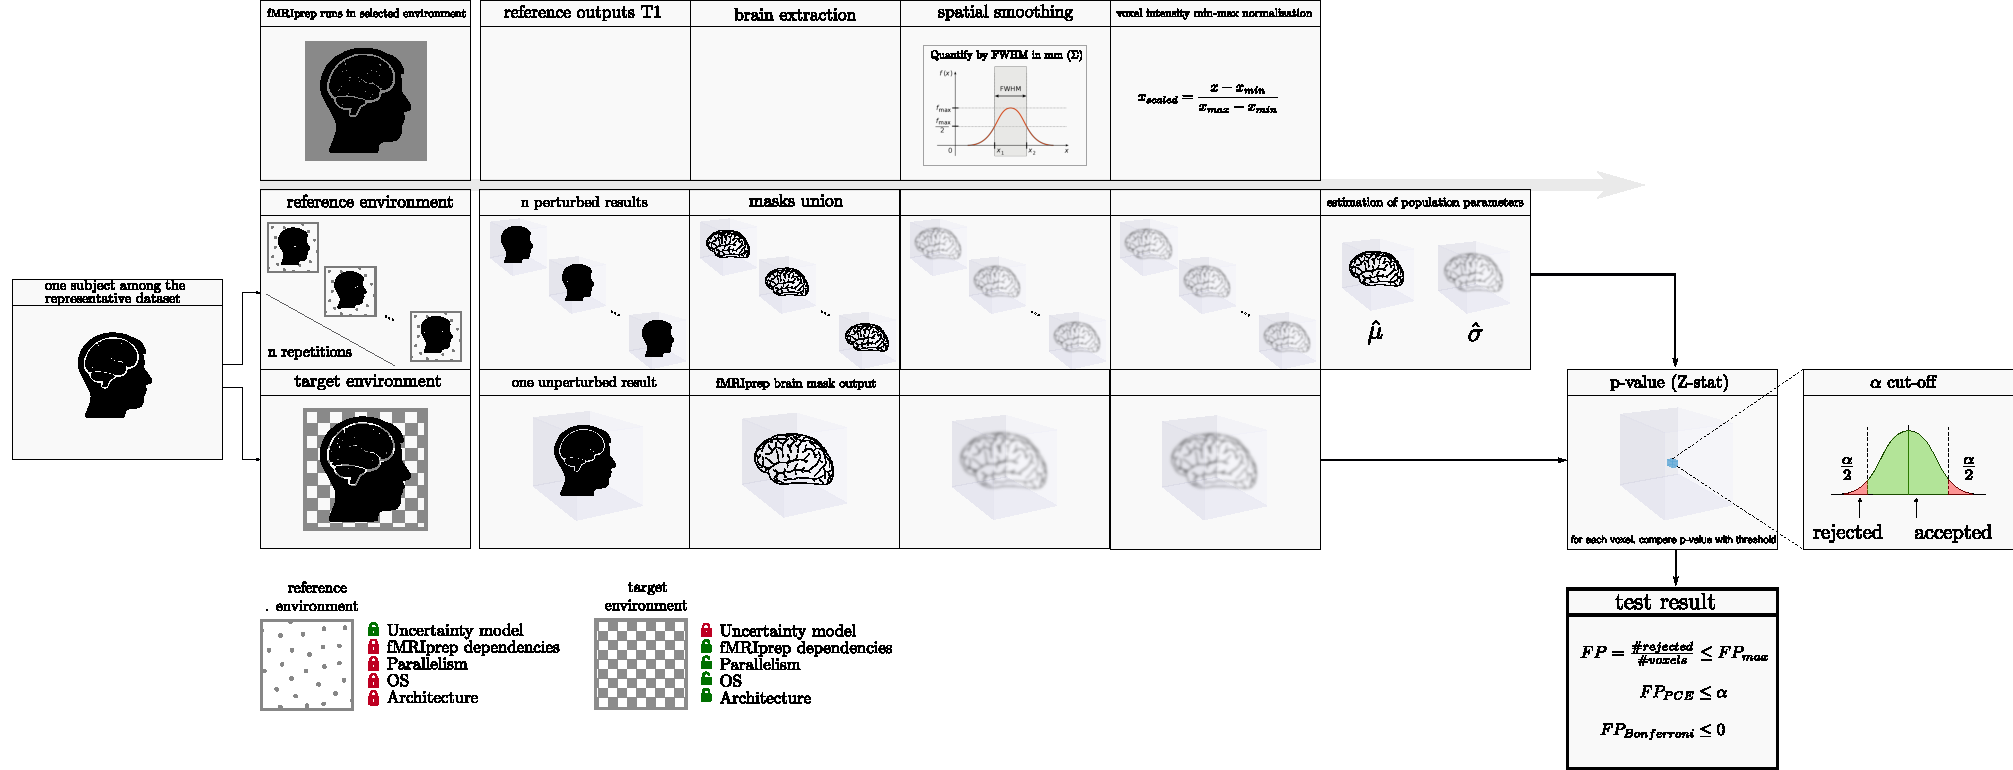
\includegraphics[width=\linewidth]{figures/stat_test_procedure.pdf}
    \caption{Test workflow.}
    \label{fig:test_workflow}
\end{figure}

\subsection{Numerical variability estimation}

To estimate the distribution of reference fMRIPrep results across execution
environments and compute $\hat \mu$ and $\hat \sigma$ (Equation~\ref{eqn:pval}), we
sample results distributions by applying three types of numerical perturbations
to the computations: (1) Random Rounding (RR), which randomly rounds function
outputs in the GNU libmath, (2) Random Seed (RS), which varies the random seed
used in fMRIPrep, and (3) Random Rounding + Random Seed (RR+RS), which applies
both previous perturbations.

Random Rounding (RR) consists in rounding the exact result of a floating-point
arithmetic operation toward the previous or next floating-point number with
equal probability~\cite{forsythe1959reprint}. RR is equivalent to applying
Monte-Carlo Arithmetic (MCA) to double-precision numbers with a virtual
precision of 53 bits and to single-precision numbers with a virtual precision of
24 bits, which was shown to accurately simulate the effect of operating system
updates on the structural pre-processing pipelines of the Human Connectome
Project (HCP) when applied to GNU libmath~\cite{salari2021accurate}. Structural
HCP pipelines consist of tools assembled from the FSL~\cite{jenkinson2012fsl}
and Freesurfer~\cite{fischl2012freesurfer} toolboxes, which makes them
conceptually very similar to the structural fMRIPrep pipeline.

RR is rigorously implemented in several tools including
CADNA~\cite{jezequel2008cadna}, Verrou~\cite{fevotte2016verrou}, and
Verificarlo~\cite{denis2016verificarlo}. However, these tools incur substantial
performance overheads which makes them difficult to use with a compute-intensive
pipeline such as fMRIPrep. In addition, only Verrou supports RR instrumentation
of GNU libmath~\cite{fevotte2019debugging}, and it does so by relying on
quadruple precision, which is not scalable to the entire fMRIPrep pipeline.
Therefore, we implemented a fast, approximate RR method by randomly adding or
removing 1 ulp (unit in the last place) to the outputs of GNU libmath functions.
Our implementation is available on \href{https://github.com/verificarlo/fuzzy}{GitHub}. 
It only
approximates RR as it applies the random perturbation to an already rounded
result instead of to the exact result as done in rigorous implementations. In
practice, computing the exact result returned by GNU libmath functions is too
expensive for our use case.

Random Seeds (RS) define pseudo-random number sequences involved in various
numerical procedures such as algorithm initialization (e.g., in k-means) or
stochastic optimization (e.g., stochastic gradient descent). In fMRIPrep, random
seeds are used in skull stripping, ANTs on linear registration, \TODO{to check}.
\TODO{https://github.com/ANTsX/ANTs/wiki/Anatomy-of-an-antsRegistration-call}
fMRIPrep provides an interface to set the random seed for all the pipeline
components except skull stripping, which we used in our experiments. RS and RR
trigger different types of variability. RR can be applied transparently to any
application while RS is more specific to the type of analysis. Conversely, RR
incurs a substantial performance overhead whereas RS does not.

\subsection{fMRIprep results preprocessing}

The non-regression test applies to the main structural derivative produced by
\fmriprep: the T1 image corrected for intensity non-uniformity using
\texttt{N4BiasFieldCorrection} from \texttt{ANTS} and transformed to template
space using
\texttt{antsRegistration}, named \texttt{desc-preproc\_T1w} in the \fmriprep
outputs and $X_k$ ($k < n$) in the remainder of this paper. In addition to the
pre-processed T1 image $X_k$, \fmriprep produces a brain mask ($B_k$), a
segmentation into grey matter, white matter and cerebro-spinal fluid tissues, as
well as probability maps for each of these tissues.

Before computing the p-values in Equation~\ref{eqn:pval}, we apply the following
pre-processing steps to $X_k$: brain masking, smoothing, and intensity
normalization. For brain masking, we mask $X_k$ with the union of the brain
masks produced across all perturbed results. We use the union of the brain masks
rather than their intersection to capture variability across $B_k$ masks. For
smoothing, we apply a spatial 3D Gaussian smoothing kernel with Full-Width at Half
Maximum (\fwhm) ranging from 0~mm to 20~mm. For intensity normalization, we apply
a min-max scaling to the smoothed intensities to scale them to [0,1].

\subsection{Handling multiple comparisons}

Handling multiple comparisons is a critical component of statistical testing in
neuroimaging given the high number of voxels tested for each 3D structural
image---typically more than 10 million~\cite{NICHOLS2007246}. The non-regression
test defined in Equation~\ref{eqn:pval} consists of independent z-tests performed
for each of the $v$ voxels of each test image, resulting in a set of $v$
p-values $p_i$, $i < v$. We corrected for multiple comparisons by adjusting the p-value
threshold. We use the classical Bonferroni correction that simply divides
$\alpha$ by the number of multiple comparisons performed. As a result, the
tested \fmriprep result is considered part of the reference distribution iif:
\begin{equation}
    \label{eq:bonferroni}
    \forall i, \quad i < v, \quad p_i < \frac{\alpha}{v}.
\end{equation}

% \begin{table}[] \centering \begin{tabular}{c|c|c|c} & Negatives & Positives &
%     \\
%          True noise  & $V_{0N}$ & $\mathbf{V_{0P}}$ & $v_0$ \\
%          True signal & $V_{1N}$ & $V_{1P}$ & $v_1$ \\
%                      & $V_N$    & ${V_P}$    & $v$ \end{tabular}
%     \caption{Cross-classification of all $v$ voxels in an image.}
%     \label{tab:cross-classification-fp} \end{table}


\subsection*{Numerical variability measure}

We computed significant bits using the \texttt{significant\_digits} package
v0.1.2 available at \url{https://github.com/verificarlo/significantdigits} that
implements the non-parametric approach described in~\cite{sohier2021confidence}.
For each bit, this method defines the significance $S^k_i$ where \(k\) is the
position of the bit in the mantissa and $X_i$ is a perturbed sample  ($i \leq
    n$). Given $Z_i=X_i/\overline{x}-1$, where $\overline{x}$ is the voxelwise average
over the perturbed results, the bit is considered significant if the absolute value of $Z_i$ is less
than $2^{-k}$:
\[S^k_i = \mathds{1}_{|Z_i |<2^{-k}}\] Then, to calculate the number of
significant bits across samples, $\hat{s_b}$, we determine the maximal index
\(k\) for which the first \(k\) bits of all \(n\) sampled results coincide with
the reference:
\[\hat{s_{b}} = \textnormal{max} \left\{ k \in \{1,2,...,p\} \textnormal{ such
        that } \forall i \in \{1,2,...,n\},\  S^{k}_{i} \textnormal{ is true } \right\} \]
where $p$ is the precision of the format ($p=16$ for int16, $p=24$ for float32).
According to~\cite{sohier2021confidence}, taking $n=30$ samples
corresponds to a confidence of 95\% and a probability of 0.9 on the estimation of $\hat{s_b}$.


\subsection{Datasets}

We selected eight test subjects from sub-datasets in OpenNeuro, representing a
diversity of age, sex, and study designs. The datasets include a motion study
with children (ds000256), a long-term memory study with young adults (ds001748),
and a motor process study with adults (ds002338). In addition, two sub-datasets
involve steps of the pipeline that can affect its reproducibility, namely
different field maps (ds001600) and non-structural images (ds001771).
Table~\ref{table:dataset_info} lists the dimension, voxels resolution, age and sex of each
subject in the dataset.

\begin{table}
    \begin{center}
        \begin{tabular}{ c|c|l|c|c|c|c|c}
            Index & Dataset  & Subject     & Dimension ($x,y,z$)         & Voxel resolution $mm^3$ ($x,y,z$) & Data type & Age  & Sex \\
            \hline
            1     & ds001600 & sub-1       & $176 \times 256 \times 256$ & $1.0 \times 1.0 \times 1.0$       & int16     & -    & -   \\
            2     & ds001771 & sub-36      & $256 \times 320 \times 320$ & $0.8 \times 0.8 \times 0.8$       & int16     & 22   & F   \\
            3     & ds000256 & sub-CTS201  & $256 \times 256 \times 256$ & $1.0 \times 1.0 \times 1.0$       & int16     & 8.68 & M   \\
            4     & ds000256 & sub-CTS210  & $224 \times 256 \times 256$ & $0.8 \times 0.8 \times 0.8$       & int16     & 7.63 & F   \\
            5     & ds001748 & sub-adult15 & $176 \times 240 \times 256$ & $1.0 \times 1.0 \times 1.0$       & float32   & 21   & M   \\
            6     & ds001748 & sub-adult16 & $176 \times 240 \times 256$ & $1.0 \times 1.0 \times 1.0$       & float32   & 21   & F   \\
            7     & ds002338 & sub-xp201   & $176 \times 512 \times 512$ & $1.0 \times 0.5 \times 0.5$       & int16     & 41   & F   \\
            8     & ds002338 & sub-xp207   & $176 \times 512 \times 512$ & $1.0 \times 0.5 \times 0.5$       & int16     & 39   & M   \\
        \end{tabular}
    \end{center}
    \caption{Dimension, voxels resolutions, age and sex of each subject in the dataset.}
    \label{table:dataset_info}
\end{table}


% \TG{report on resolution and data types}

% \begin{itemize}
%     \item \st{Describe Openneuro project}
%     \item \st{Describe each dataset}
% \end{itemize}

\subsection{Computing infrastructure}

We processed the dataset using the Narval cluster managed by Calcul Qu\'ebec and
Compute Canada. With our job submission parameters, we could access 1,145
computing nodes with 64 cores per node and 2 $\times$ AMD Rome 7532 @ 2.40 GHz
256M cache L3. We executed \fmriprep in a Singularity container built from a
Docker image available on dockerhub \texttt{yohanchatelain/fmriprep-fuzzy:20.2.1}.
The container image used Ubuntu \texttt{16.04.6 LTS}, GNU
libc/libmath \texttt{2.23}, kernel \texttt{4.18.0-372.19.1}
\texttt{.el8\_6.x86\_64}, and fMRIPrep version \texttt{20.2.1}. We disabled
multi-threading in fMRIPrep, fixed the random seed for skull stripping as well
as in fMRIPrep (RR condition only), and verified that in these conditions
fMRIPrep results were bit-to-bit reproducible.

\section{Results}

We computed 30 perturbed results for each of the 8 subjects and each of the 3
perturbations (RR, RS, RR+RS). We also computed a reference, unperturbed IEEE
result for each subject using a random seed of 42. For each perturbation we
measured the uncertainty of fMRIPrep in terms of significant bits, and we
built the non-regression test using different values of FWHM smoothing and confidence level.

\subsection{Measured uncertainty}

Overall, the three types of perturbations (RR, RS, RR+RS) created uncertainties
of comparable magnitude (Figure~\ref{fig:numerical-uncertainty}), with intensity
standard deviations ranging from 0 to 0.04 and significant bits ranging from 3
bits to 10 bits. Overall the measured uncertainty is high, with mean significant bits
ranging from 3 bits to 10 bits out of the 12 bits available in the data. Numerically, \fmriprep 
appears to be highly sensitive to the numerical or random seed perturbation. We also observe 
substantial discrepancies among subjects. For a given smoothing kernel size, 
the number of significant bits frequently varies in the ratio of 1 to 3 among subjects. 
Overall, smoothing tends to reduce numerical uncertainty, however, this behavior is in general not monotonous
and varies across subjects. 

The uncertainty measured across perturbed samples showed regional variations
compatible with anatomical features (Figure~\ref{fig:uncertainty_sub_1}). 
In
particular, uncertainty was maximal at the border of the brain mask, and it was
overall higher in the gray matter than in the white matter. This is consistent
with previous observations of numerical uncertainty in structural brain image
analysis~\cite{salari2021accurate}. In addition, uncertainty was also maximal in
some cortical regions, suggesting that non-linear registration may be unstable
in these regions. Our non-regression test will therefore be more tolerant in
these regions. \TODO{use Gaussian sigbits and update text accordingly}


\begin{figure}
    \centering
    \includegraphics[width=\linewidth]{figures/stats.pdf}
    \caption{Voxel-wise means of mean, standard deviation and significant bits
        measured across n=30 perturbed samples for 3 types of perturbations and 8
        subjects. For each subject, we computed statistics in the union of the brain
        masks among n=30 perturbed samples.}
    \label{fig:numerical-uncertainty}
\end{figure}

\begin{landscape}
    \begin{figure}

        \vspace*{-2cm}
        \centering
        %% sub 1
        \begin{subfigure}[b][][c]{0.01\paperwidth} 1 \vspace*{-45pt} \end{subfigure}
        \begin{subfigure}[t]{0.2\paperheight}
            \centering
            IEEE (T1 intensity)
            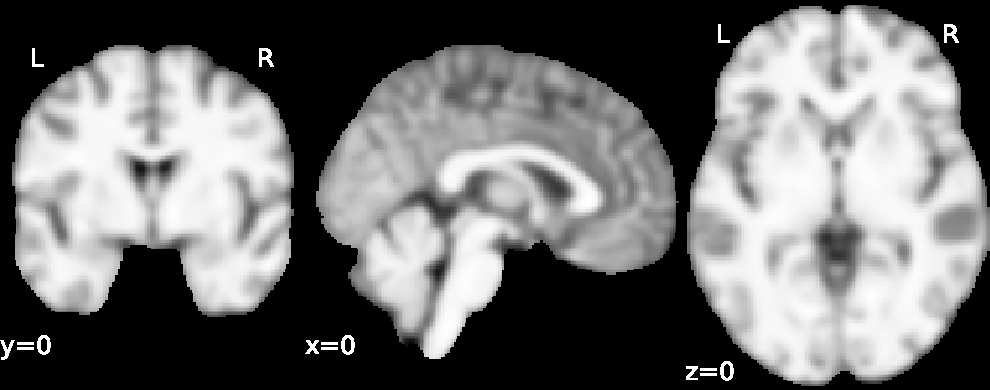
\includegraphics[width=\textwidth]{figures/ieee_T1/fwhm_5/ieee_ds001600_sub-1.pdf}
        \end{subfigure}
        \begin{subfigure}[t]{0.2\paperheight}
            \centering
            RR (significant bits)
            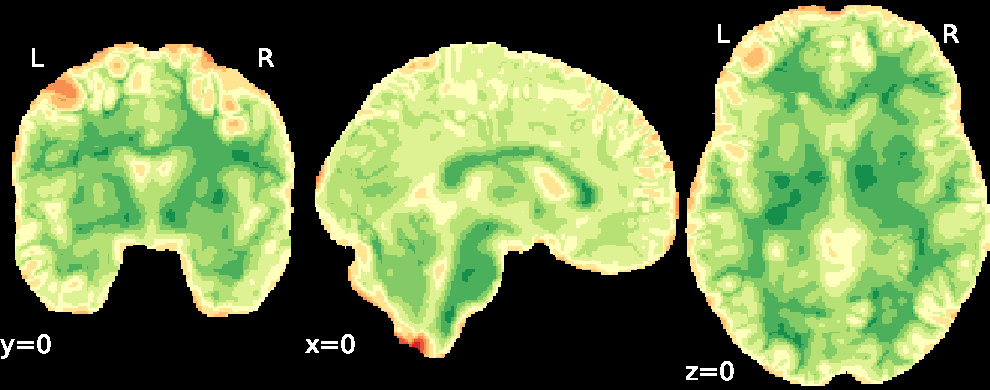
\includegraphics[width=\textwidth]{figures/sig/fwhm_5/rr_ds001600_sub-1_sig.pdf}
        \end{subfigure}
        \begin{subfigure}[t]{0.2\paperheight}
            \centering
            RS (significant bits)
            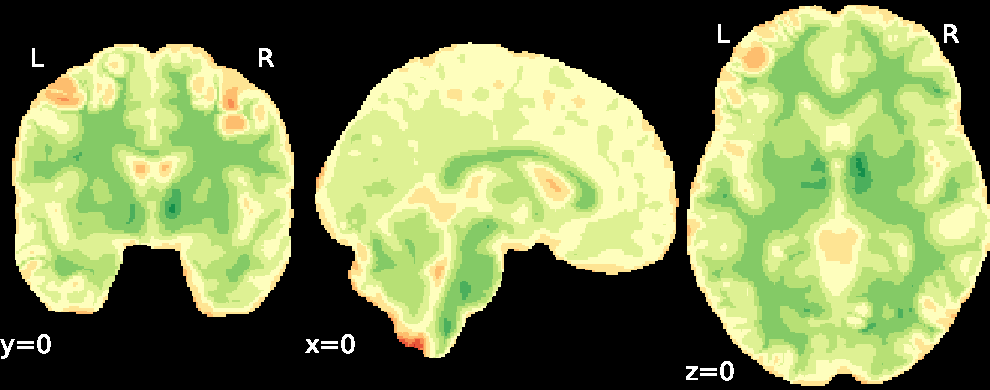
\includegraphics[width=\textwidth]{figures/sig/fwhm_5/rs_ds001600_sub-1_sig.pdf}
        \end{subfigure}
        \begin{subfigure}[t]{0.2\paperheight}
            \centering
            RS (significant bits)
            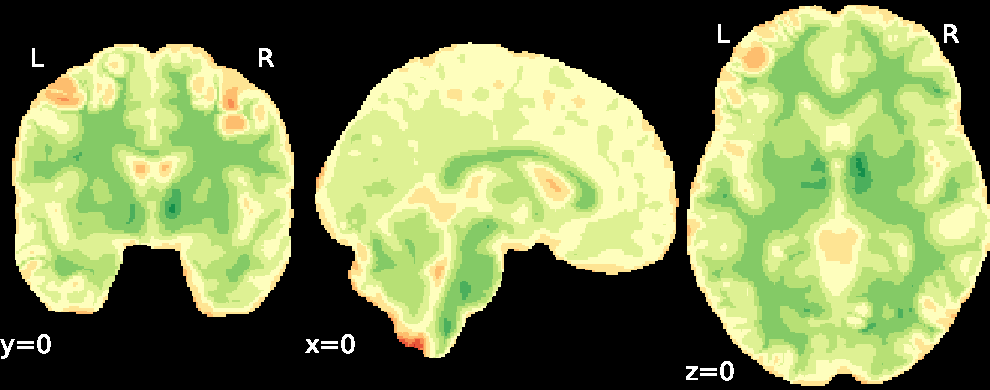
\includegraphics[width=\textwidth]{figures/sig/fwhm_5/rs_ds001600_sub-1_sig.pdf}
        \end{subfigure}
        %% sub 2
        \begin{subfigure}[b][][c]{0.01\paperwidth} 2 \vspace*{15pt} \end{subfigure}
        \begin{subfigure}[t]{0.2\paperheight}
            \centering
            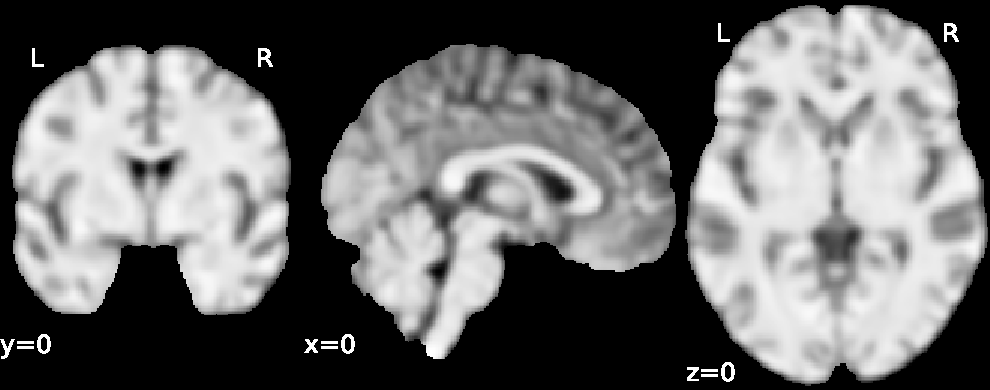
\includegraphics[width=\textwidth]{figures/ieee_T1/fwhm_5/ieee_ds001771_sub-36.pdf}
        \end{subfigure}
        \begin{subfigure}[t]{0.2\paperheight}
            \centering
            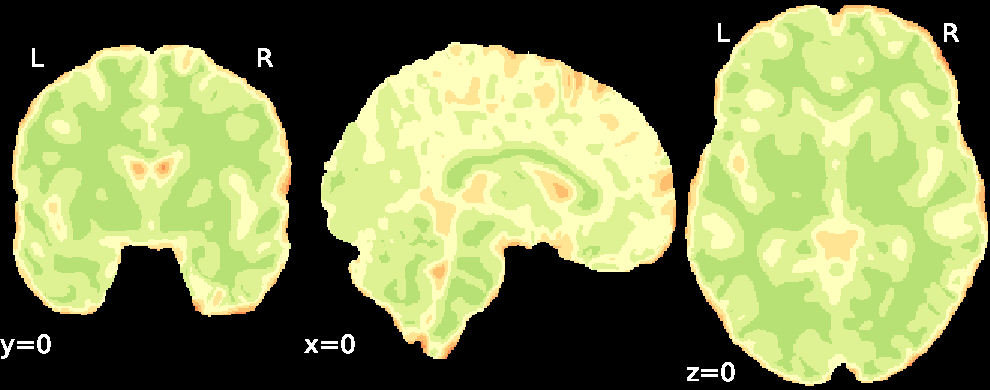
\includegraphics[width=\textwidth]{figures/sig/fwhm_5/rr_ds001771_sub-36_sig.pdf}
        \end{subfigure}
        \begin{subfigure}[t]{0.2\paperheight}
            \centering
            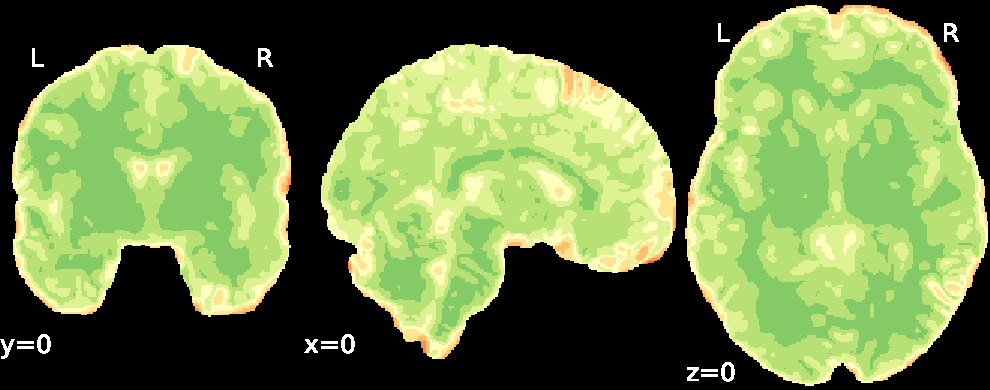
\includegraphics[width=\textwidth]{figures/sig/fwhm_5/rs_ds001771_sub-36_sig.pdf}
        \end{subfigure}
        \begin{subfigure}[t]{0.2\paperheight}
            \centering
            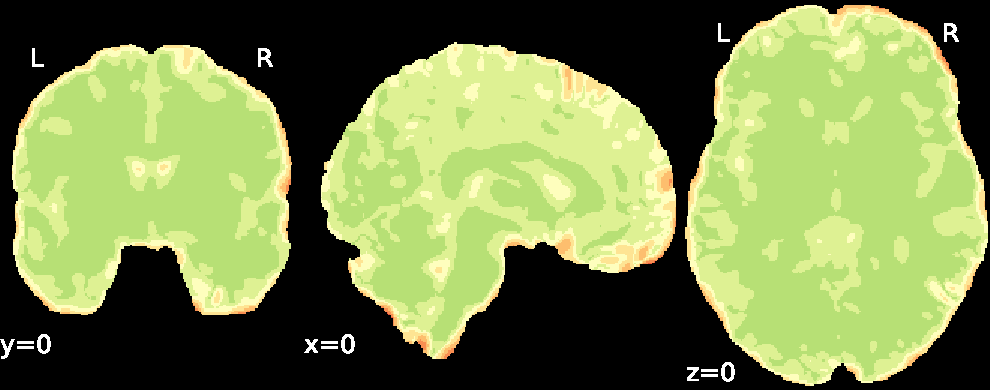
\includegraphics[width=\textwidth]{figures/sig/fwhm_5/rr.rs_ds001771_sub-36_sig.pdf}
        \end{subfigure} \\
        %% sub 3
        \begin{subfigure}[b][][c]{0.01\paperwidth} 3 \vspace*{15pt} \end{subfigure}
        \begin{subfigure}[t]{0.2\paperheight}
            \centering
            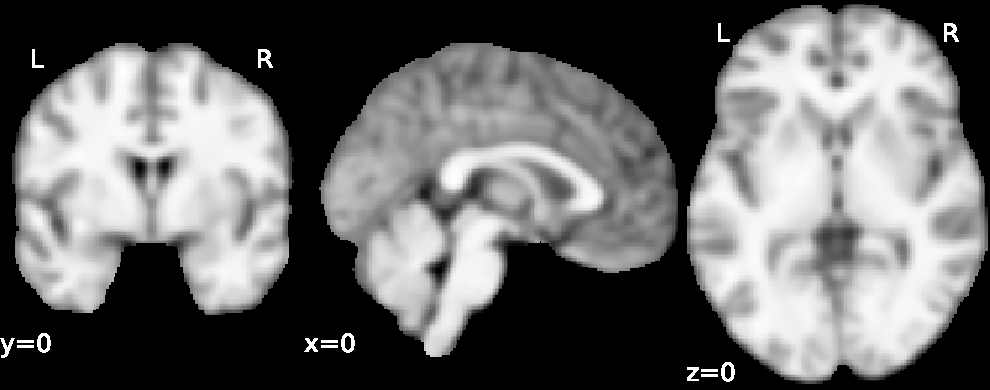
\includegraphics[width=\textwidth]{figures/ieee_T1/fwhm_5/ieee_ds000256_sub-CTS201.pdf}
        \end{subfigure}
        \begin{subfigure}[t]{0.2\paperheight}
            \centering
            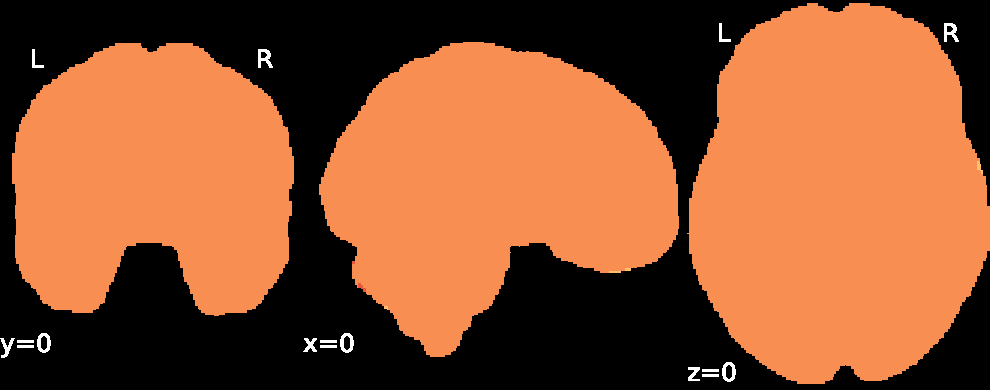
\includegraphics[width=\textwidth]{figures/sig/fwhm_5/rr_ds000256_sub-CTS201_sig.pdf}
        \end{subfigure}
        \begin{subfigure}[t]{0.2\paperheight}
            \centering
            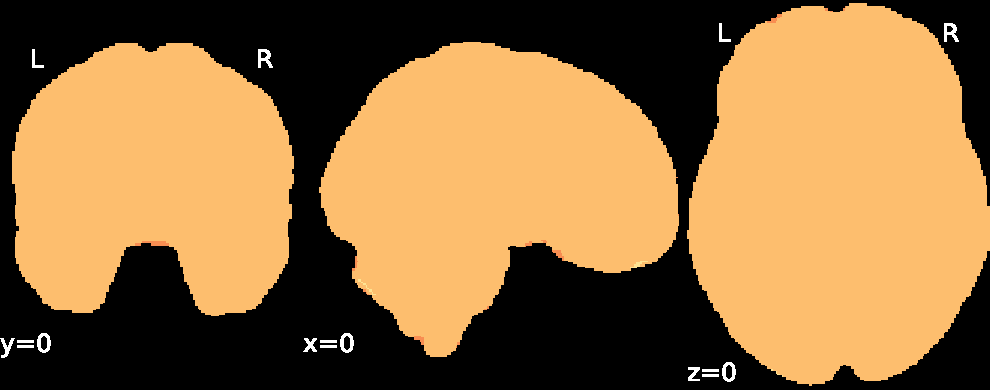
\includegraphics[width=\textwidth]{figures/sig/fwhm_5/rs_ds000256_sub-CTS201_sig.pdf}
        \end{subfigure}
        \begin{subfigure}[t]{0.2\paperheight}
            \centering
            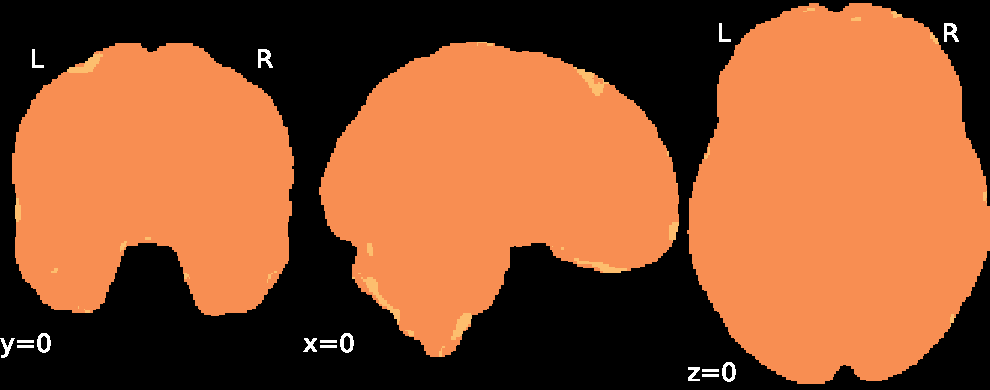
\includegraphics[width=\textwidth]{figures/sig/fwhm_5/rr.rs_ds000256_sub-CTS201_sig.pdf}
        \end{subfigure} \\
        %% sub 4
        \begin{subfigure}[b][][c]{0.01\paperwidth} 4 \vspace*{15pt} \end{subfigure}
        \begin{subfigure}[t]{0.2\paperheight}
            \centering
            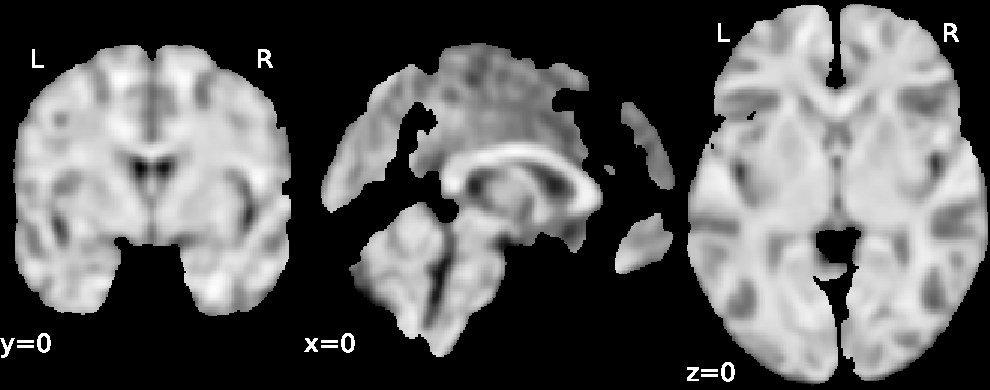
\includegraphics[width=\textwidth]{figures/ieee_T1/fwhm_5/ieee_ds000256_sub-CTS210.pdf}
        \end{subfigure}
        \begin{subfigure}[t]{0.2\paperheight}
            \centering
            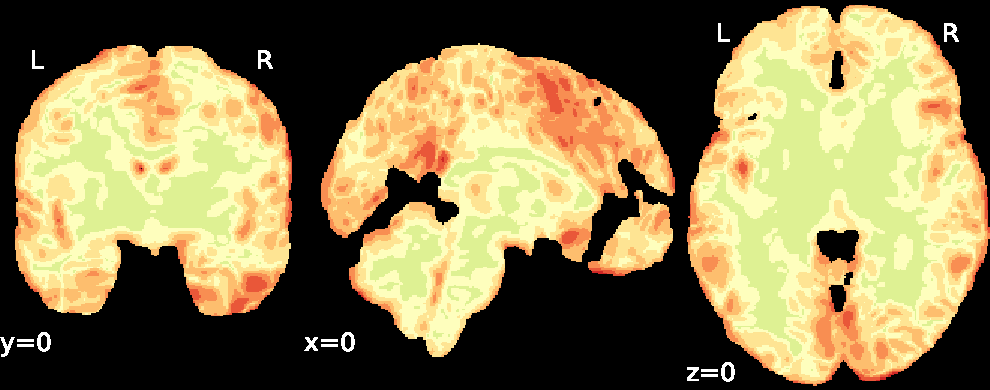
\includegraphics[width=\textwidth]{figures/sig/fwhm_5/rr_ds000256_sub-CTS210_sig.pdf}
        \end{subfigure}
        \begin{subfigure}[t]{0.2\paperheight}
            \centering
            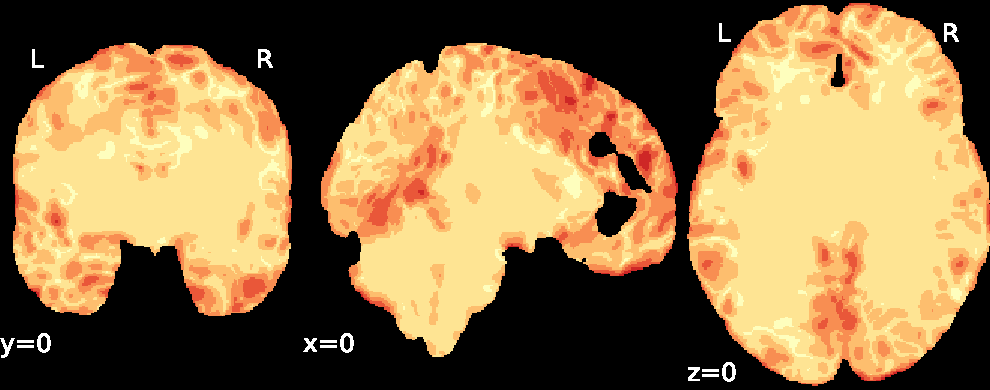
\includegraphics[width=\textwidth]{figures/sig/fwhm_5/rs_ds000256_sub-CTS210_sig.pdf}
        \end{subfigure}
        \begin{subfigure}[t]{0.2\paperheight}
            \centering
            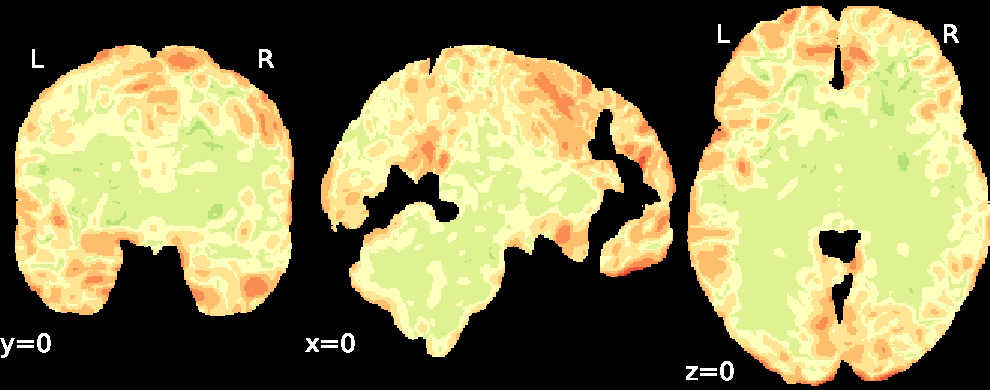
\includegraphics[width=\textwidth]{figures/sig/fwhm_5/rr.rs_ds000256_sub-CTS210_sig.pdf}
        \end{subfigure} \\
        %% sub 5
        \begin{subfigure}[b][][c]{0.01\paperwidth} 5 \vspace*{15pt} \end{subfigure}
        \begin{subfigure}[t]{0.2\paperheight}
            \centering
            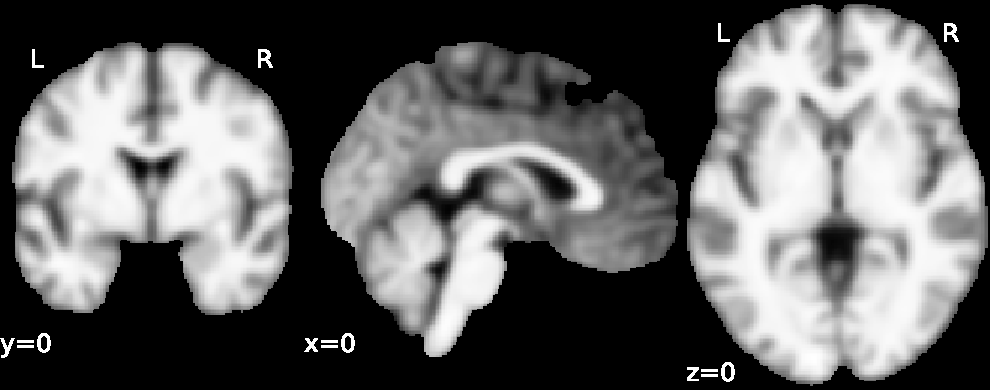
\includegraphics[width=\textwidth]{figures/ieee_T1/fwhm_5/ieee_ds001748_sub-adult15.pdf}
        \end{subfigure}
        \begin{subfigure}[t]{0.2\paperheight}
            \centering
            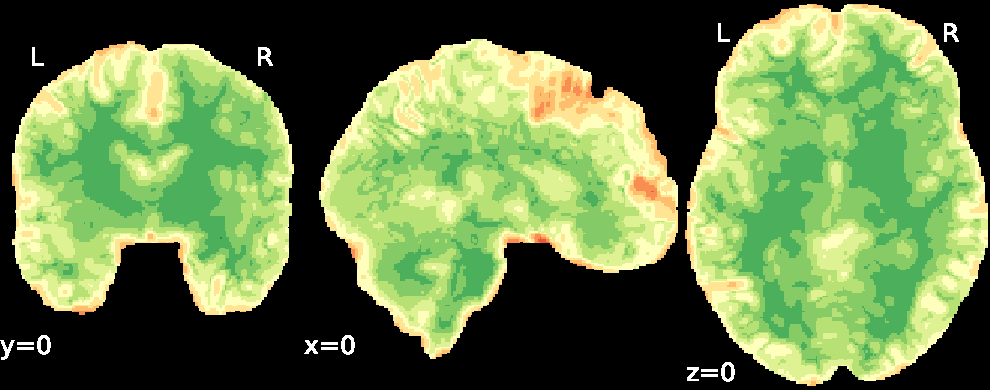
\includegraphics[width=\textwidth]{figures/sig/fwhm_5/rr_ds001748_sub-adult15_sig.pdf}
        \end{subfigure}
        \begin{subfigure}[t]{0.2\paperheight}
            \centering
            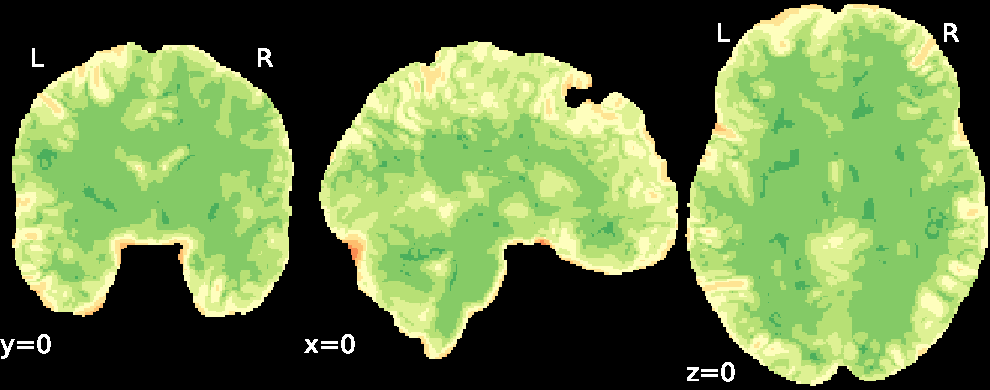
\includegraphics[width=\textwidth]{figures/sig/fwhm_5/rs_ds001748_sub-adult15_sig.pdf}
        \end{subfigure}
        \begin{subfigure}[t]{0.2\paperheight}
            \centering
            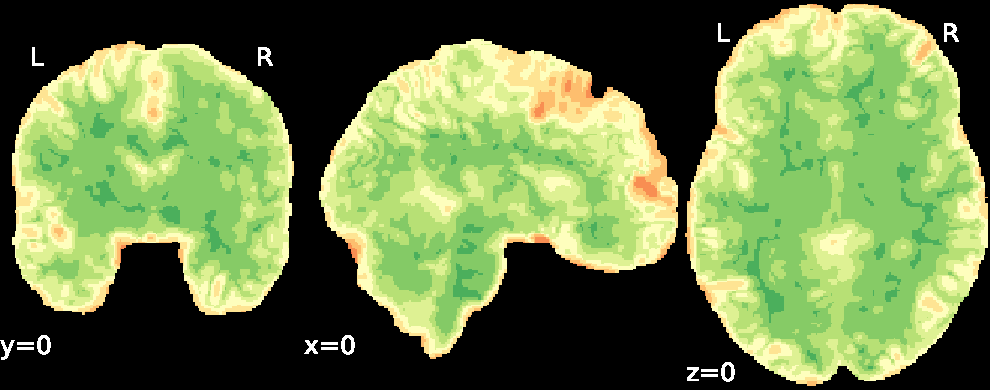
\includegraphics[width=\textwidth]{figures/sig/fwhm_5/rr.rs_ds001748_sub-adult15_sig.pdf}
        \end{subfigure} \\
        %% sub 6
        \begin{subfigure}[b][][c]{0.01\paperwidth} 6 \vspace*{15pt} \end{subfigure}
        \begin{subfigure}[t]{0.2\paperheight}
            \centering
            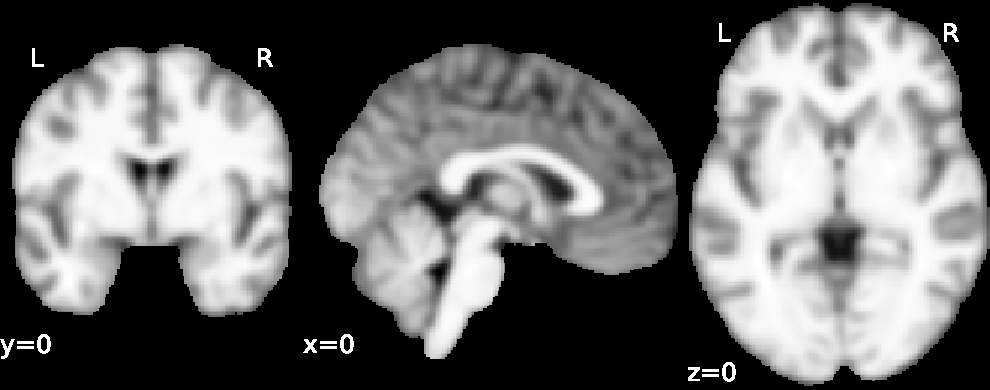
\includegraphics[width=\textwidth]{figures/ieee_T1/fwhm_5/ieee_ds001748_sub-adult16.pdf}
        \end{subfigure}
        \begin{subfigure}[t]{0.2\paperheight}
            \centering
            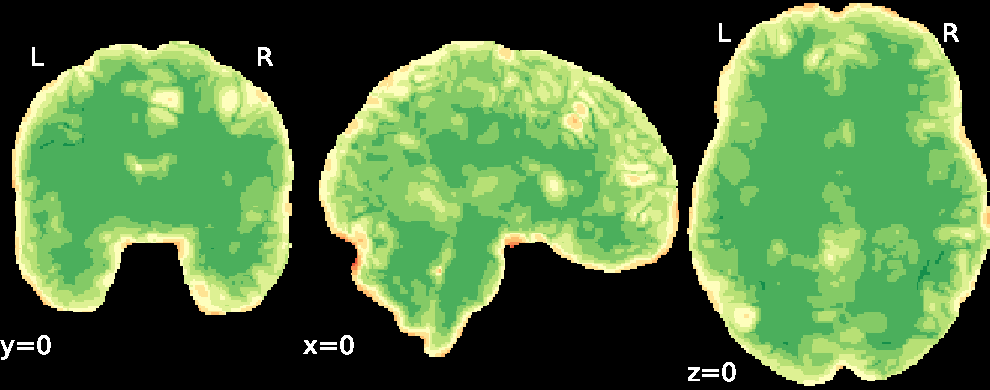
\includegraphics[width=\textwidth]{figures/sig/fwhm_5/rr_ds001748_sub-adult16_sig.pdf}
        \end{subfigure}
        \begin{subfigure}[t]{0.2\paperheight}
            \centering
            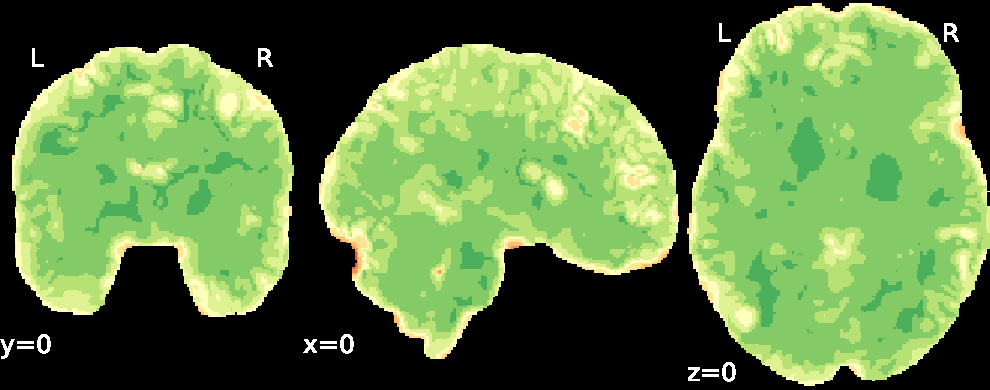
\includegraphics[width=\textwidth]{figures/sig/fwhm_5/rs_ds001748_sub-adult16_sig.pdf}
        \end{subfigure}
        \begin{subfigure}[t]{0.2\paperheight}
            \centering
            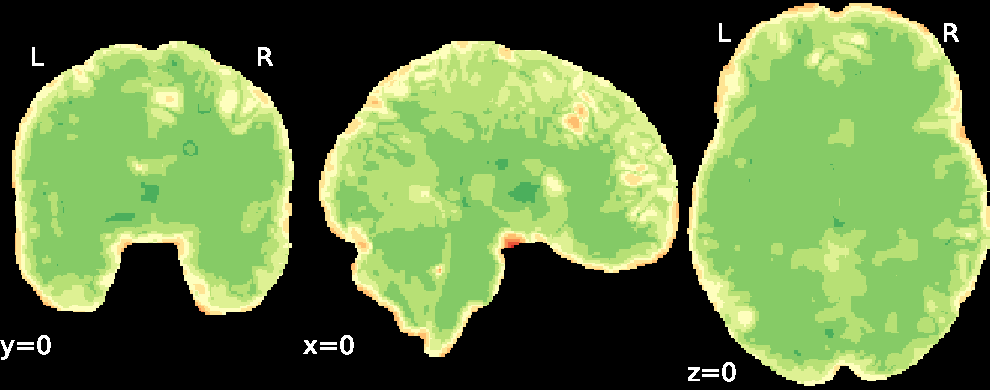
\includegraphics[width=\textwidth]{figures/sig/fwhm_5/rr.rs_ds001748_sub-adult16_sig.pdf}
        \end{subfigure} \\
        %% sub 7
        \begin{subfigure}[b][][c]{0.01\paperwidth} 7 \vspace*{15pt} \end{subfigure}
        \begin{subfigure}[t]{0.2\paperheight}
            \centering
            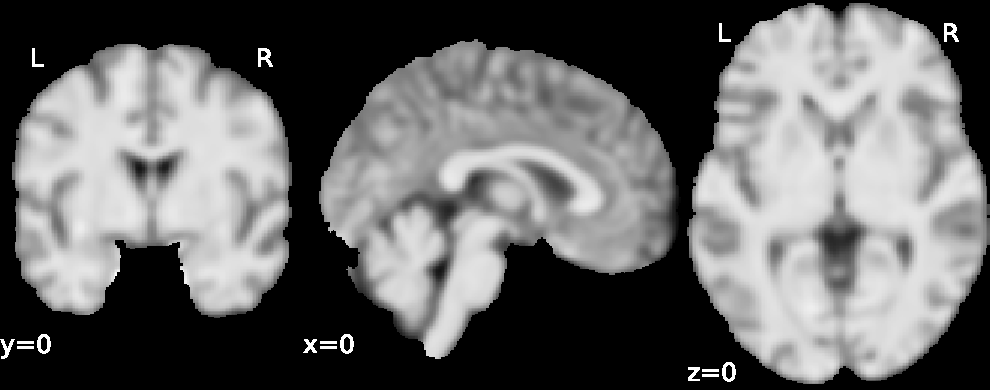
\includegraphics[width=\textwidth]{figures/ieee_T1/fwhm_5/ieee_ds002338_sub-xp201.pdf}
        \end{subfigure}
        \begin{subfigure}[t]{0.2\paperheight}
            \centering
            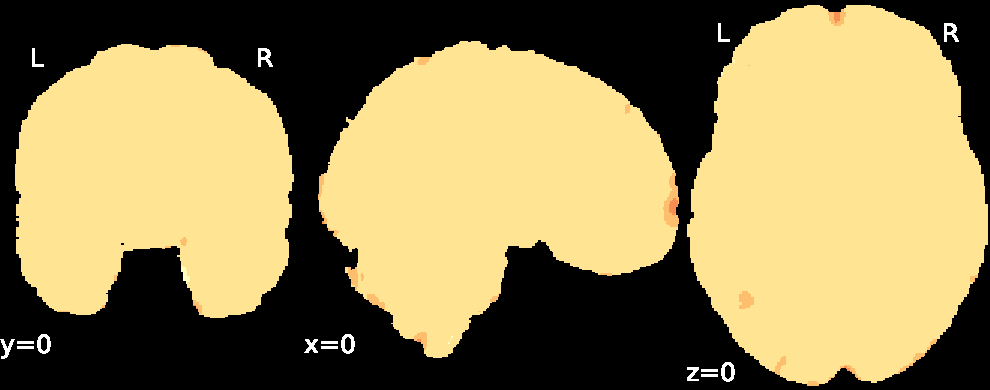
\includegraphics[width=\textwidth]{figures/sig/fwhm_5/rr_ds002338_sub-xp201_sig.pdf}
        \end{subfigure}
        \begin{subfigure}[t]{0.2\paperheight}
            \centering
            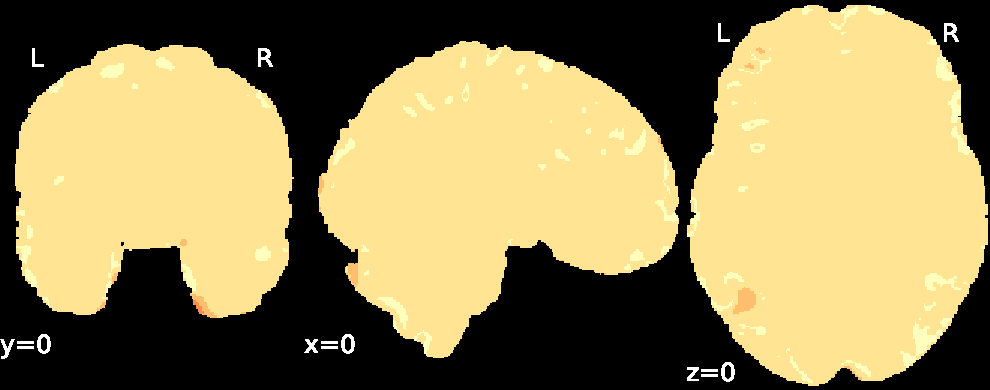
\includegraphics[width=\textwidth]{figures/sig/fwhm_5/rs_ds002338_sub-xp201_sig.pdf}
        \end{subfigure}
        \begin{subfigure}[t]{0.2\paperheight}
            \centering
            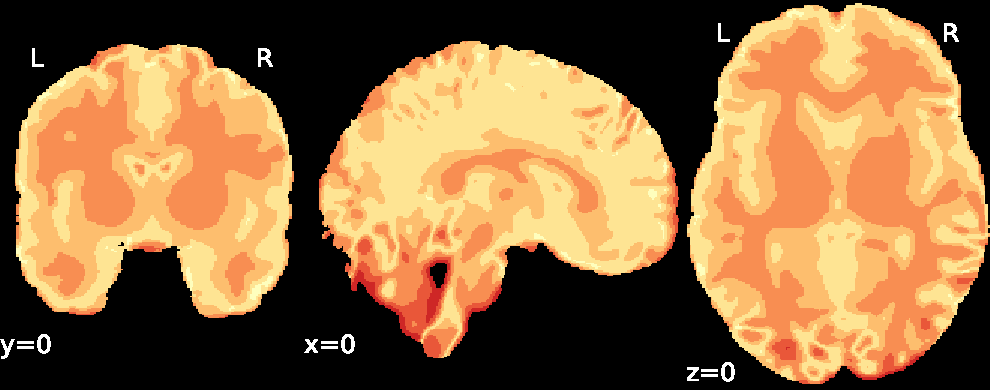
\includegraphics[width=\textwidth]{figures/sig/fwhm_5/rr.rs_ds002338_sub-xp201_sig.pdf}
        \end{subfigure} \\
        %% sub 8 
        \begin{subfigure}[b][][c]{0.01\paperwidth} 8 \vspace*{15pt} \end{subfigure}
        \begin{subfigure}[t]{0.2\paperheight}
            \centering
            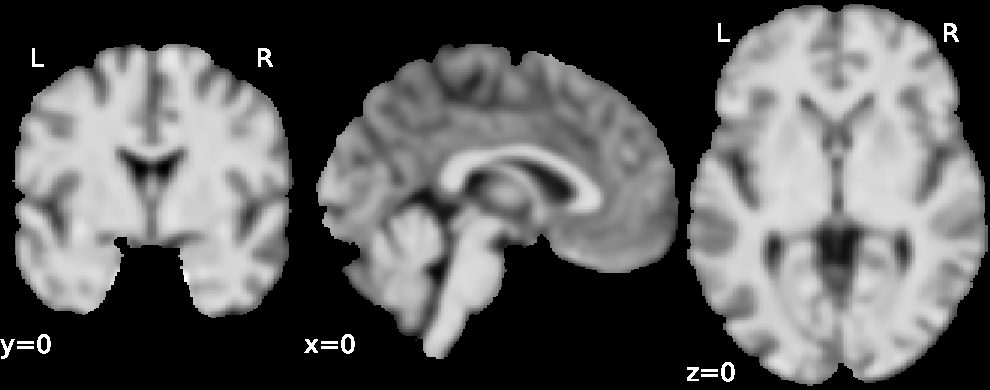
\includegraphics[width=\textwidth]{figures/ieee_T1/fwhm_5/ieee_ds002338_sub-xp207.pdf}
        \end{subfigure}
        \begin{subfigure}[t]{0.2\paperheight}
            \centering
            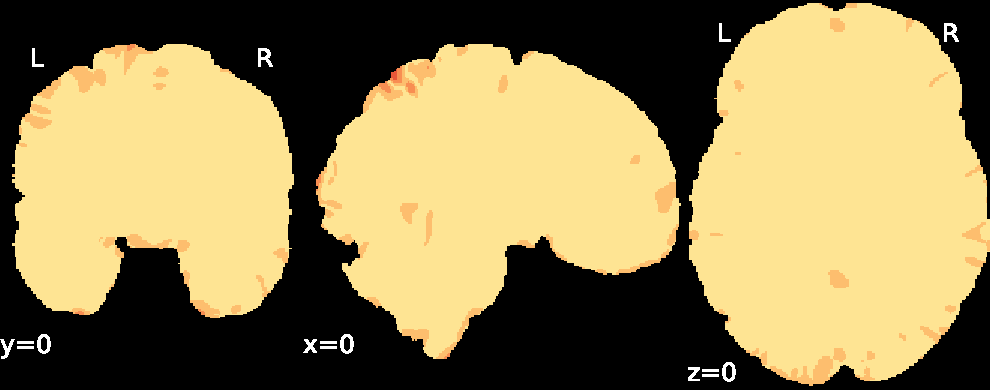
\includegraphics[width=\textwidth]{figures/sig/fwhm_5/rr_ds002338_sub-xp207_sig.pdf}
        \end{subfigure}
        \begin{subfigure}[t]{0.2\paperheight}
            \centering
            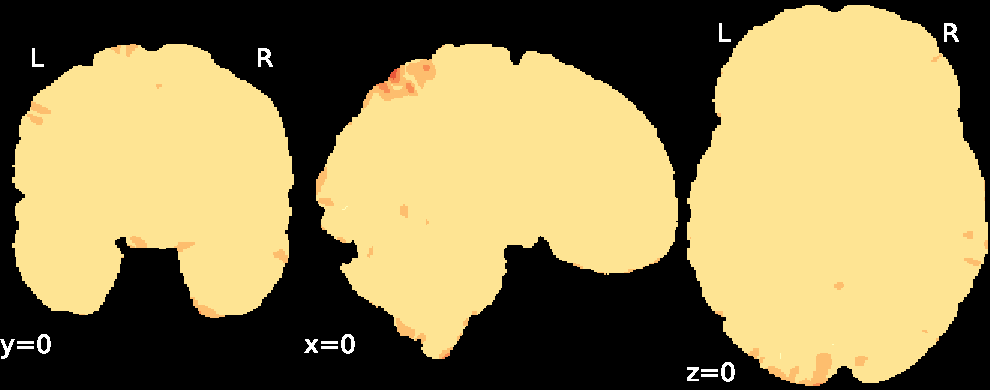
\includegraphics[width=\textwidth]{figures/sig/fwhm_5/rs_ds002338_sub-xp207_sig.pdf}
        \end{subfigure}
        \begin{subfigure}[t]{0.2\paperheight}
            \centering
            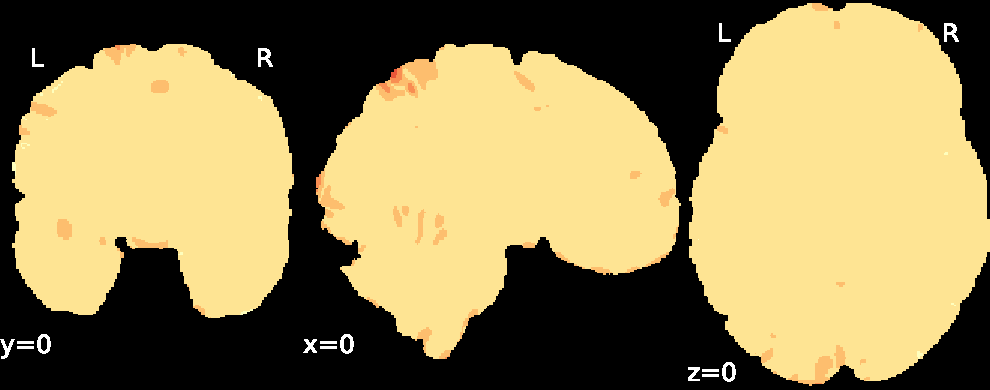
\includegraphics[width=\textwidth]{figures/sig/fwhm_5/rr.rs_ds002338_sub-xp207_sig.pdf}
        \end{subfigure} \\
        \hspace*{6cm} 0 \tikz[baseline=(current bounding box.south)]{
            \draw[left color=red, right color=green!50!black, middle color=yellow]
            (0,0) rectangle (8,0.3);} 12 bits
        \caption{Uncertainty measured for subjects 1 to 8 (from top to bottom) across n=30 for
            (from right to left) IEEE, RR, RS and RR+RS perturbed samples with a spatial smoothing applied (FWHM=5mm). }
        \label{fig:uncertainty_sub_1}

    \end{figure}
\end{landscape}


\subsection{Non-regression test evaluations}

\paragraph{Leave-one-out evaluation.} We implemented a ``leave-one-out" (LOO)
evaluation by constructing the non-regression test $n$ times for $n-1$ perturbed results
and applying it to the remaining perturbed result. We model the LOO test
using a binomial variable $B(n,1-\alpha)$
where $n$ is the number of repetitions and $1-\alpha$ is
the probability of success of a repetition. Under $H_0$ for all voxels, we 
expect the following
bound to be verified:
\[
    1-F(\mathds{1}_n;n,1-\alpha) \leq \alpha_0
\]
where $F(x;n,p)$ is the cumulative distribution function of the Binomial law $B(n,p)$, and 
$\alpha_0=0.05$.

We applied leave-one-out validation for
different  confidence values (1-$\alpha$) and different FWHM  values for the
3 types of perturbations (Figure~\ref{fig:loo_bonferroni}). As expected, tests
become increasingly permissive for increasing values of $\alpha$ (reduced
confidence) and increasing values of FWHM. As previously observed, the 3 perturbation types 
behave similarly. For each subject, $\alpha$ and FWHM values exist such that 
the LOO test passes. However, these values importantly vary across subjects, presumably
due to heterogeneous data quality. To pass the LOO
test with $\alpha=0.05$ for RR perturbations,  
subjects 2, 6, 7 and 8 require a smoothing size of FWHM=\TODO{10}mm and
subjects 3, 5 require FWHM=15mm. Subjects 1 and 4 never pass the LOO test 
at this confidence level.   

% For each type of perturbation, we
% define "best operating values" $\alpha^\star$ and $\fwhm^\star$ for these parameters
% such that:
% \begin{equation}
%     (\alpha^\star, \fwhm^\star) = \min\left(\underset{(\alpha, \fwhm)}{\mathrm{argmax}}\left( S(\alpha,\fwhm)\right)\right),
% \end{equation}
% where $S(\alpha, \fwhm)$ is the number of subjects that pass the test for
% $\alpha$ and $\fwhm$ and the minimum is determined using the lexicographic
% order on $A \times F$ where $A$ is the set of all $\alpha$ values and $F$ is the
% set of all FWHM values. $\alpha^\star$ is the minimum value of $\alpha$ for which
% the maximal number of subjects pass the test, and $\fwhm^\star$ is the minimal
% smoothing kernel size such that the maximal number of subjects pass the test
% with $\alpha^\star$. \TG{comment on $\alpha^\star$ and $\fwhm^\star$ values.}

% It can be
% noted that among the 8 tested subjects, subject 210 never passes the test for RR
% or RS perturbations, and only passed the test for $\alpha^\star=0.2$ and
% $\fwhm^\star=20mm$ for the RR+RS perturbation. This is due to the fact that for
% many voxels in this subject's image, the confidence interval resulting from a
% Gaussian fit of the intensity distribution across perturbed samples does not
% properly reflect the distribution. A visual inspection of the image did not
% show any particular image artifact (e.g., motion) or atypical anatomical feature
% (e.g., unusually large ventricles) that could explain such variations. Finally,
% as detailed in Appendix~\ref{appendix:multiple-comparison-tests}, the other
% tested methods for multiple comparison corrections led to similar conclusions.



\begin{figure}
    \centering
    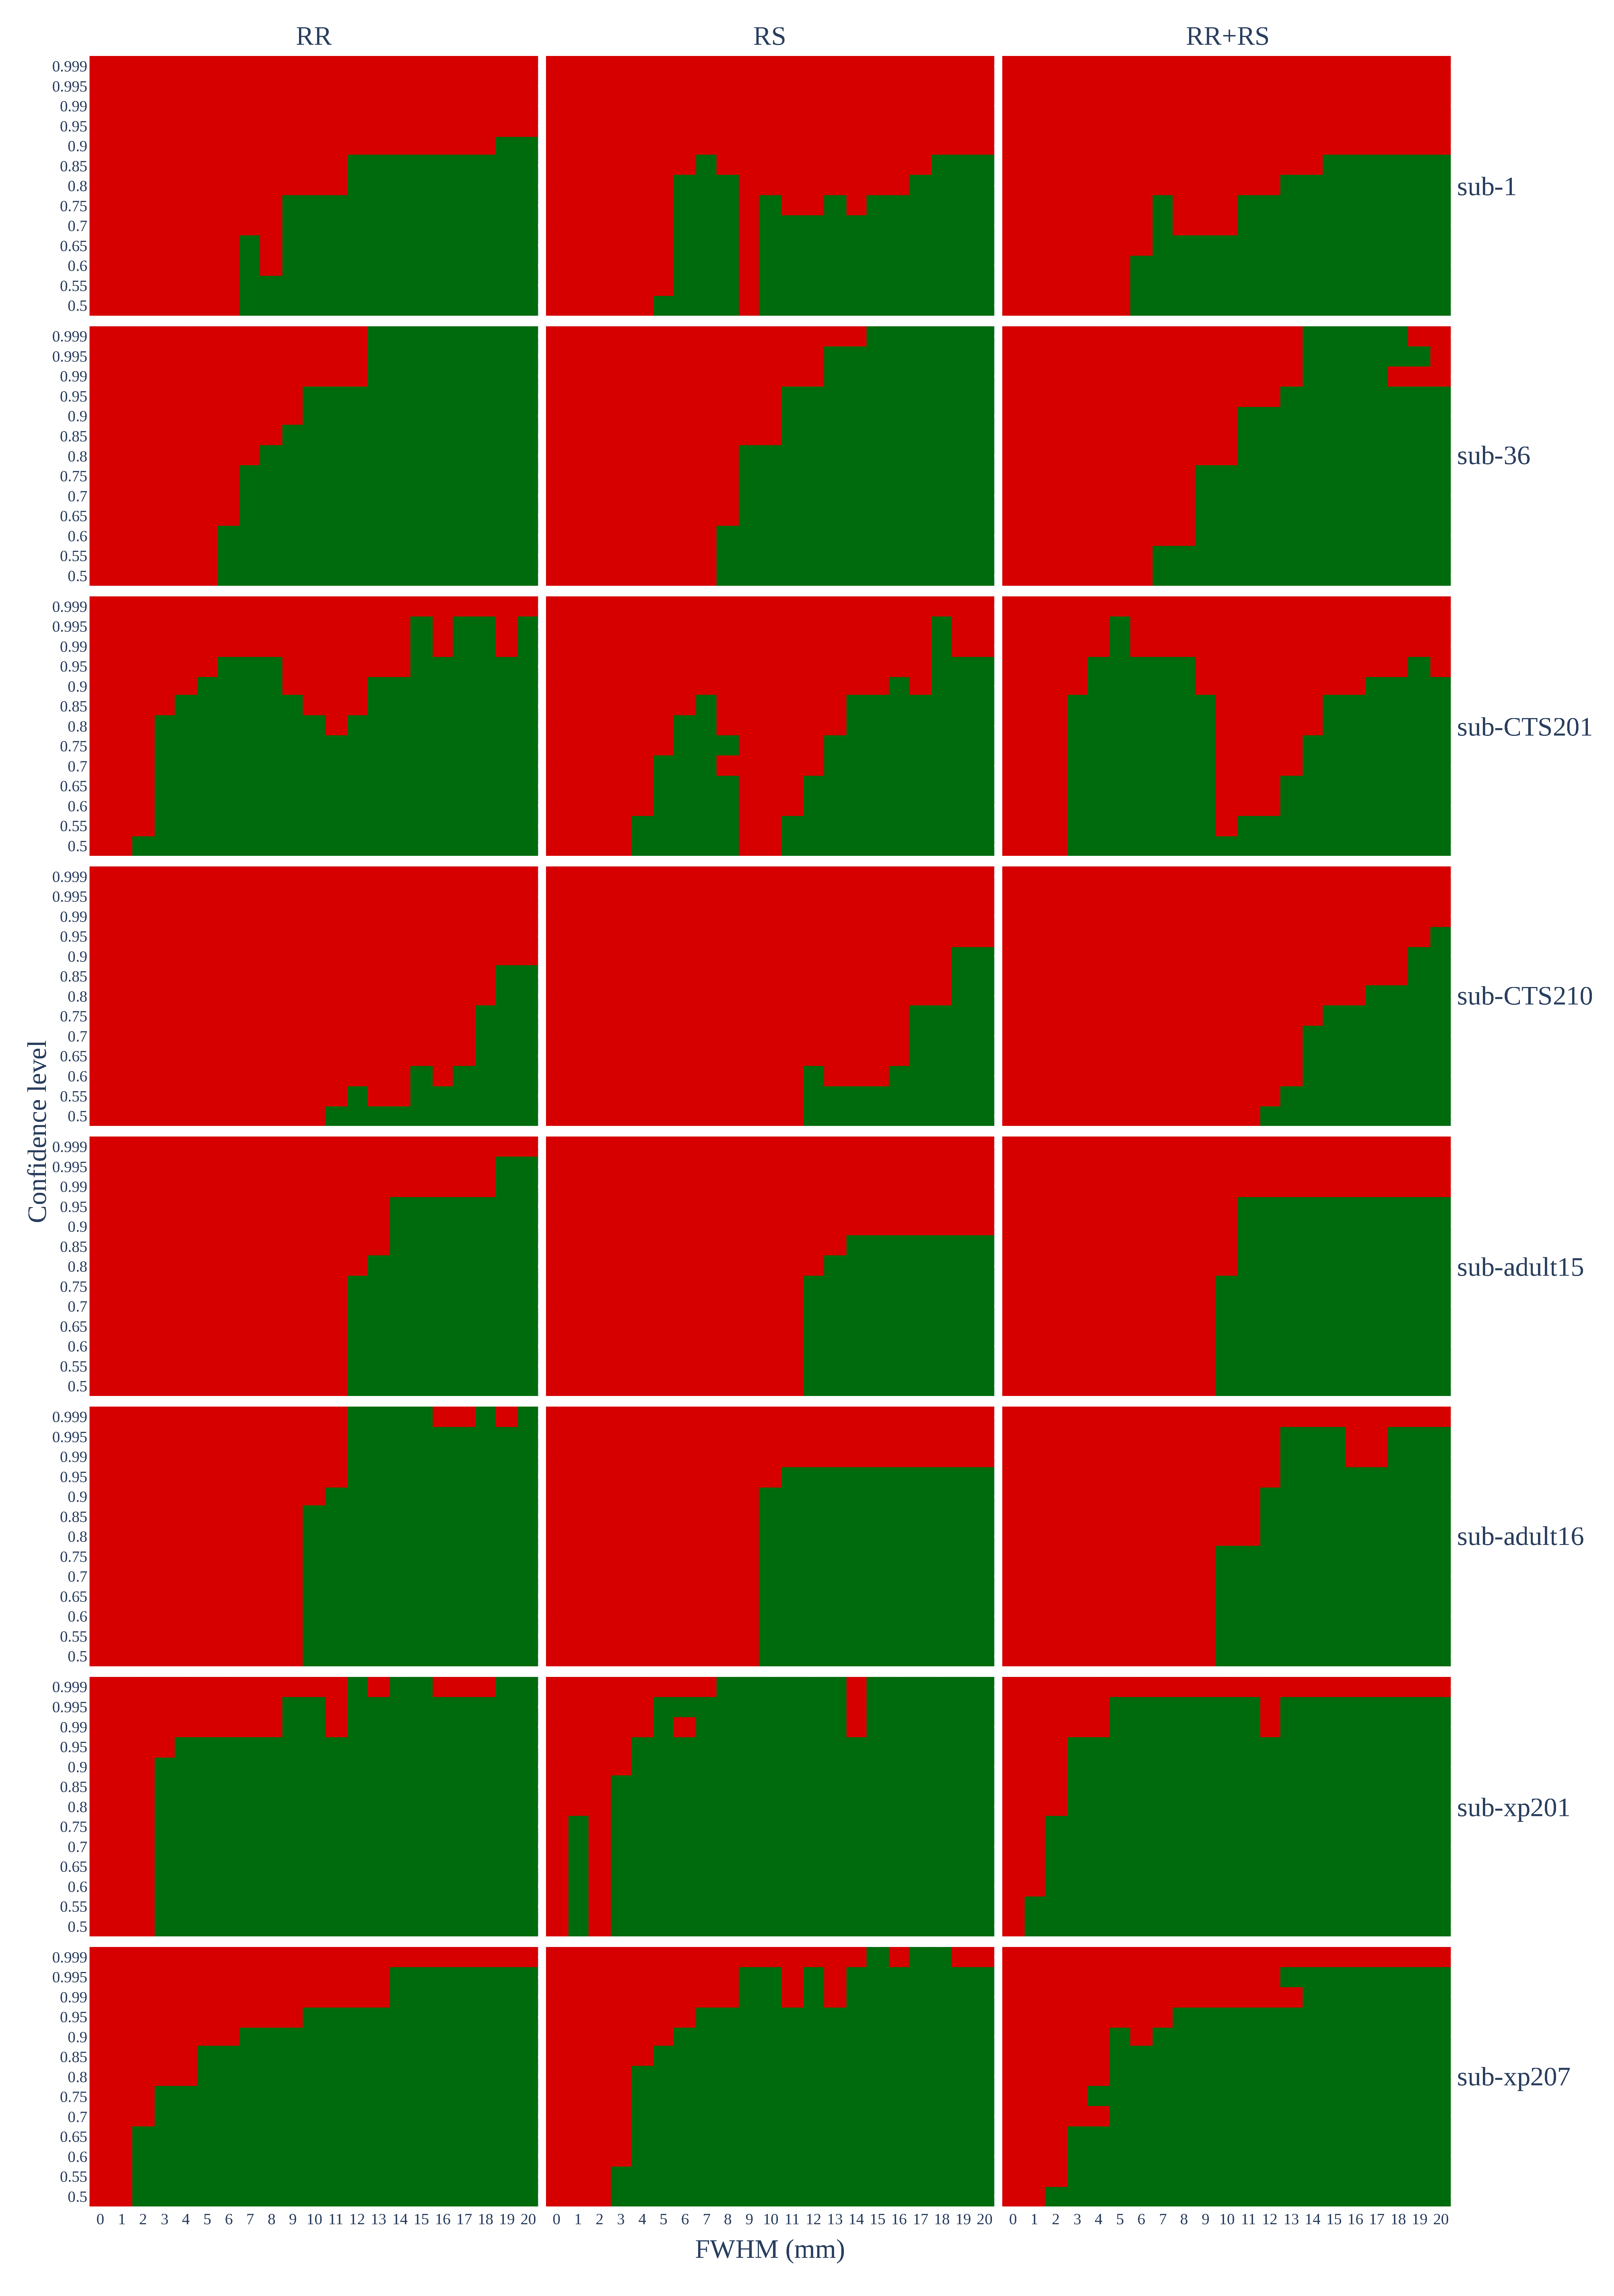
\includegraphics[width=\linewidth]{figures/exclude_mct_fwe_bonferroni.pdf}
    \caption{Leave-one-out evaluation for non-regression tests.
        Binomial one-tailed test with a confidence level at 95\%.
        Red: failed the test. Green: passed the test.}
    \label{fig:loo_bonferroni}
\end{figure}


\paragraph{IEEE check.} We check that the result computed without random perturbations
passes the corrected and uncorrected tests. 
Figure~\ref{fig:ieee-check}.

\paragraph{Corrupted template check.}


% \begin{figure}
%     \centering
%     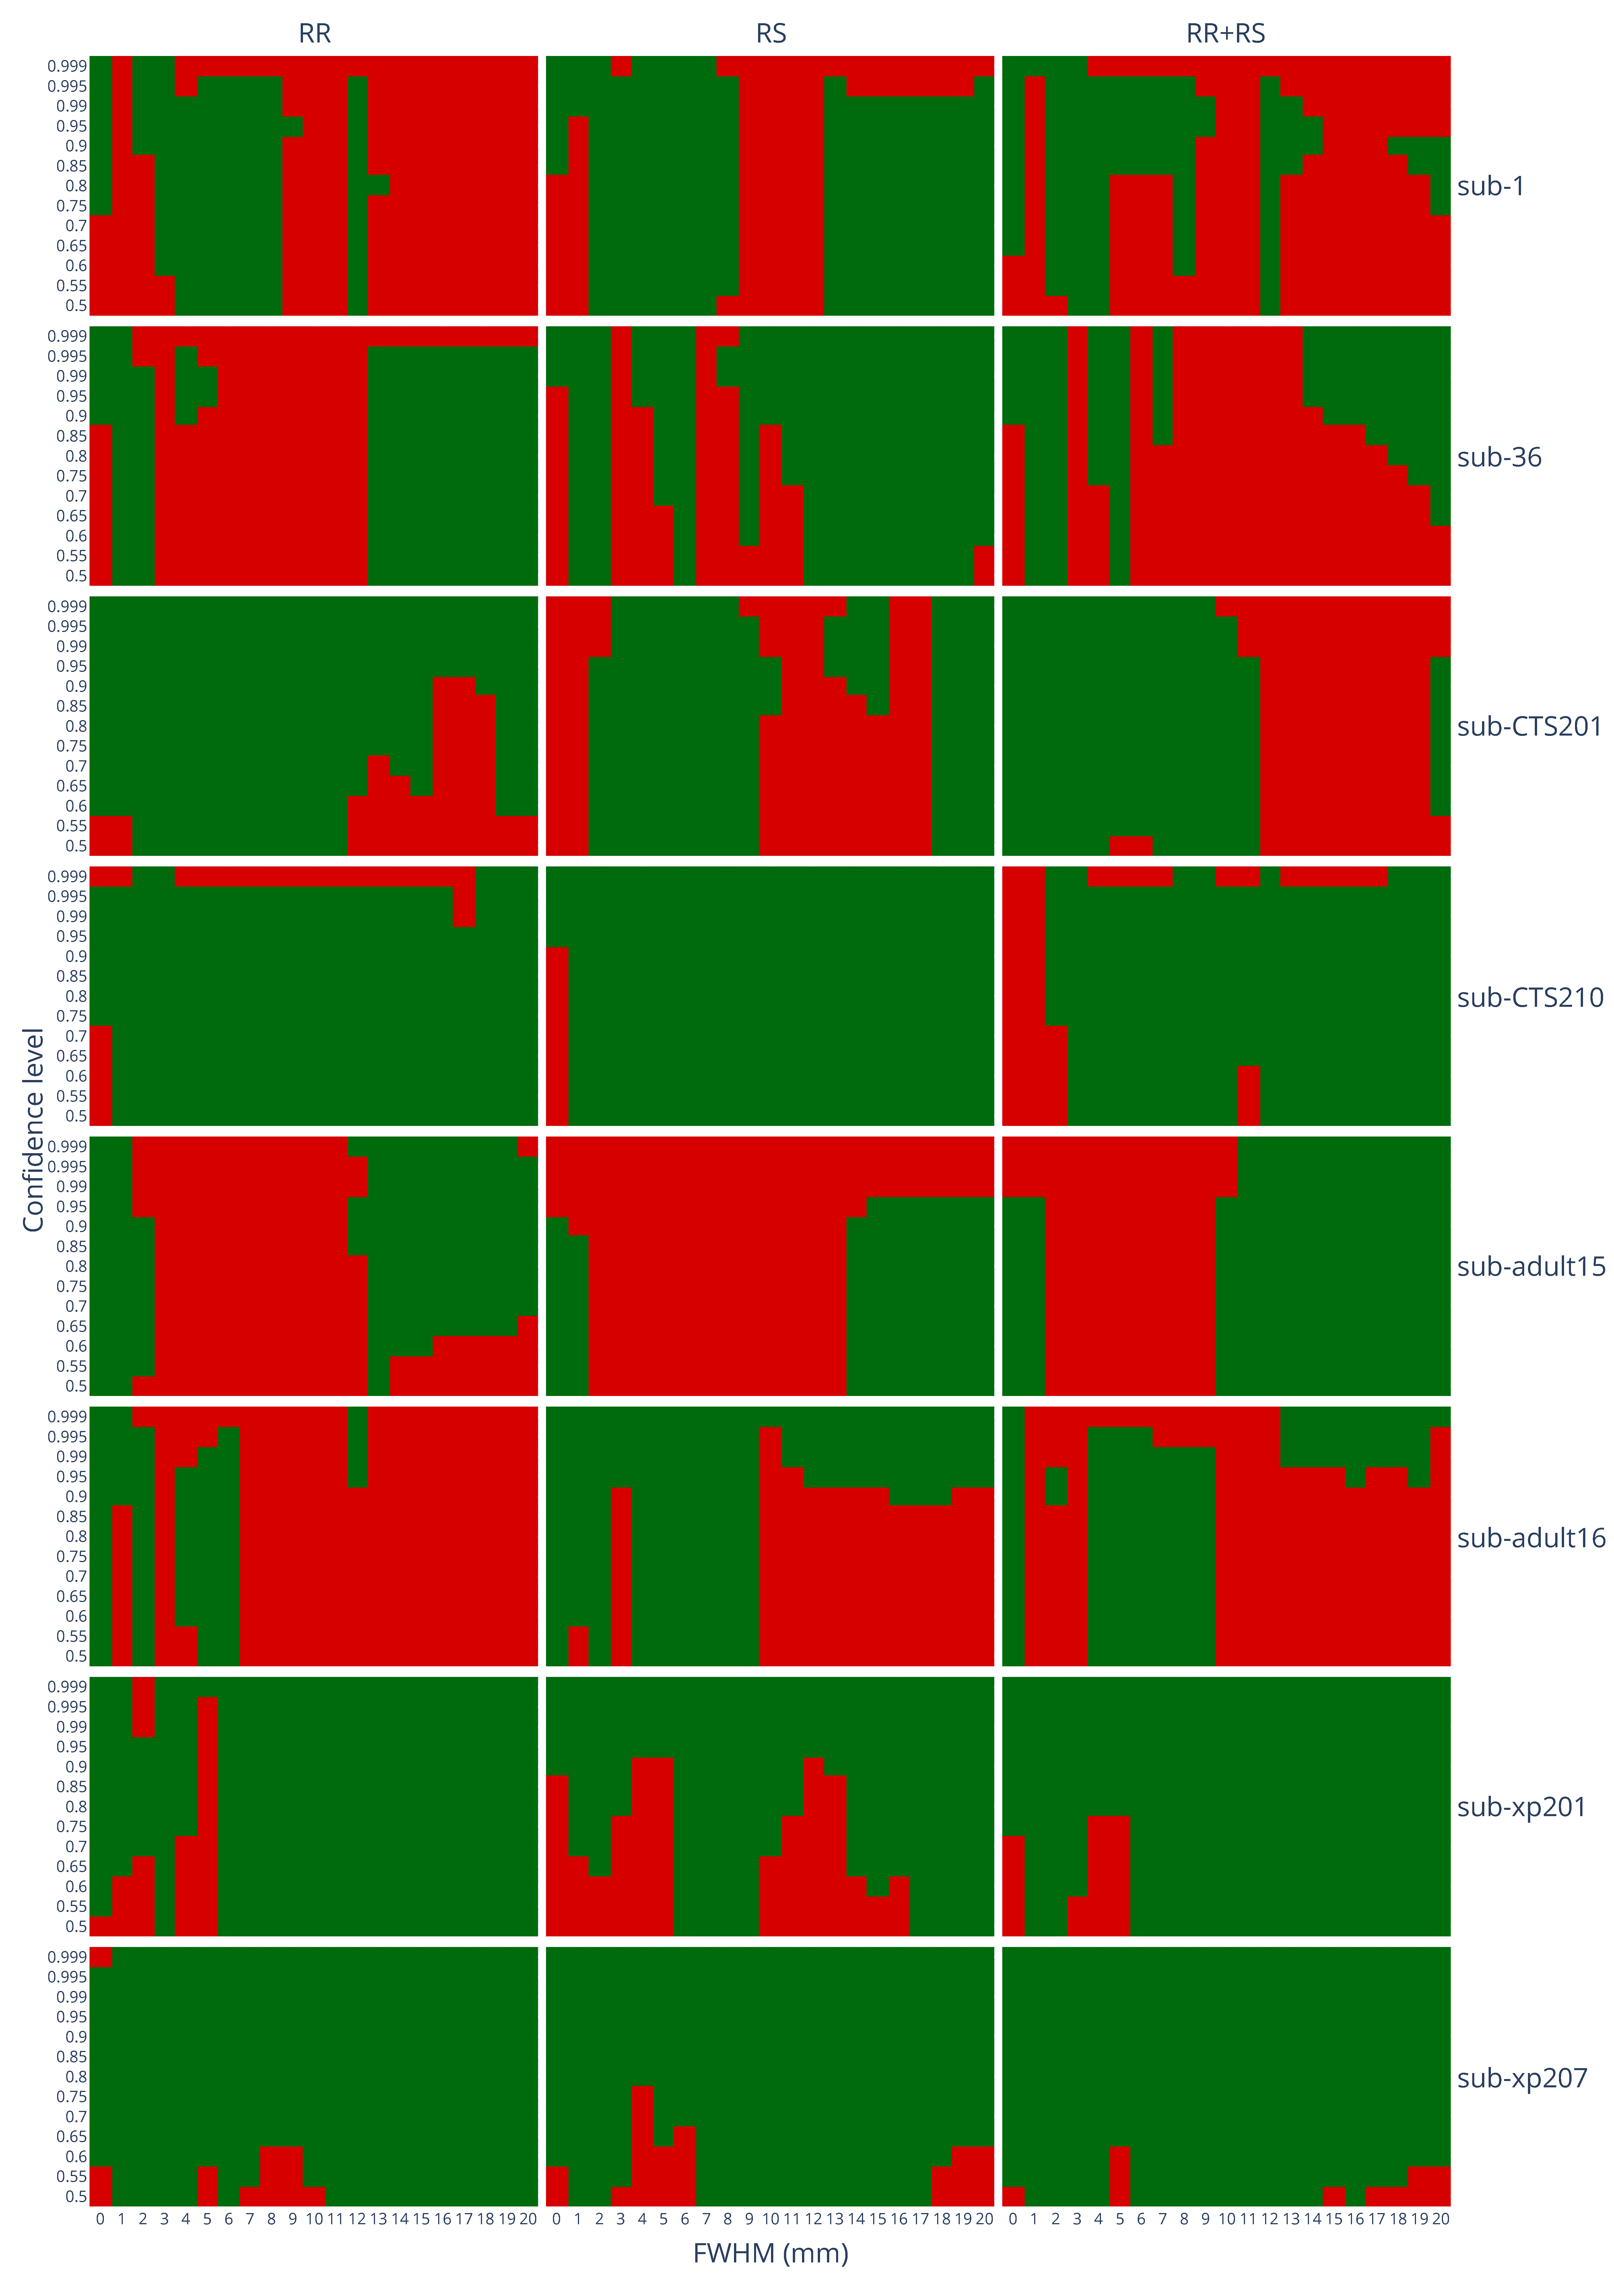
\includegraphics[width=\linewidth]{figures/ieee_pce.pdf}
%     \caption{IEEE check for uncorrected $\alpha$ threshold.}
% \end{figure}

% \begin{figure}
%     \centering
%     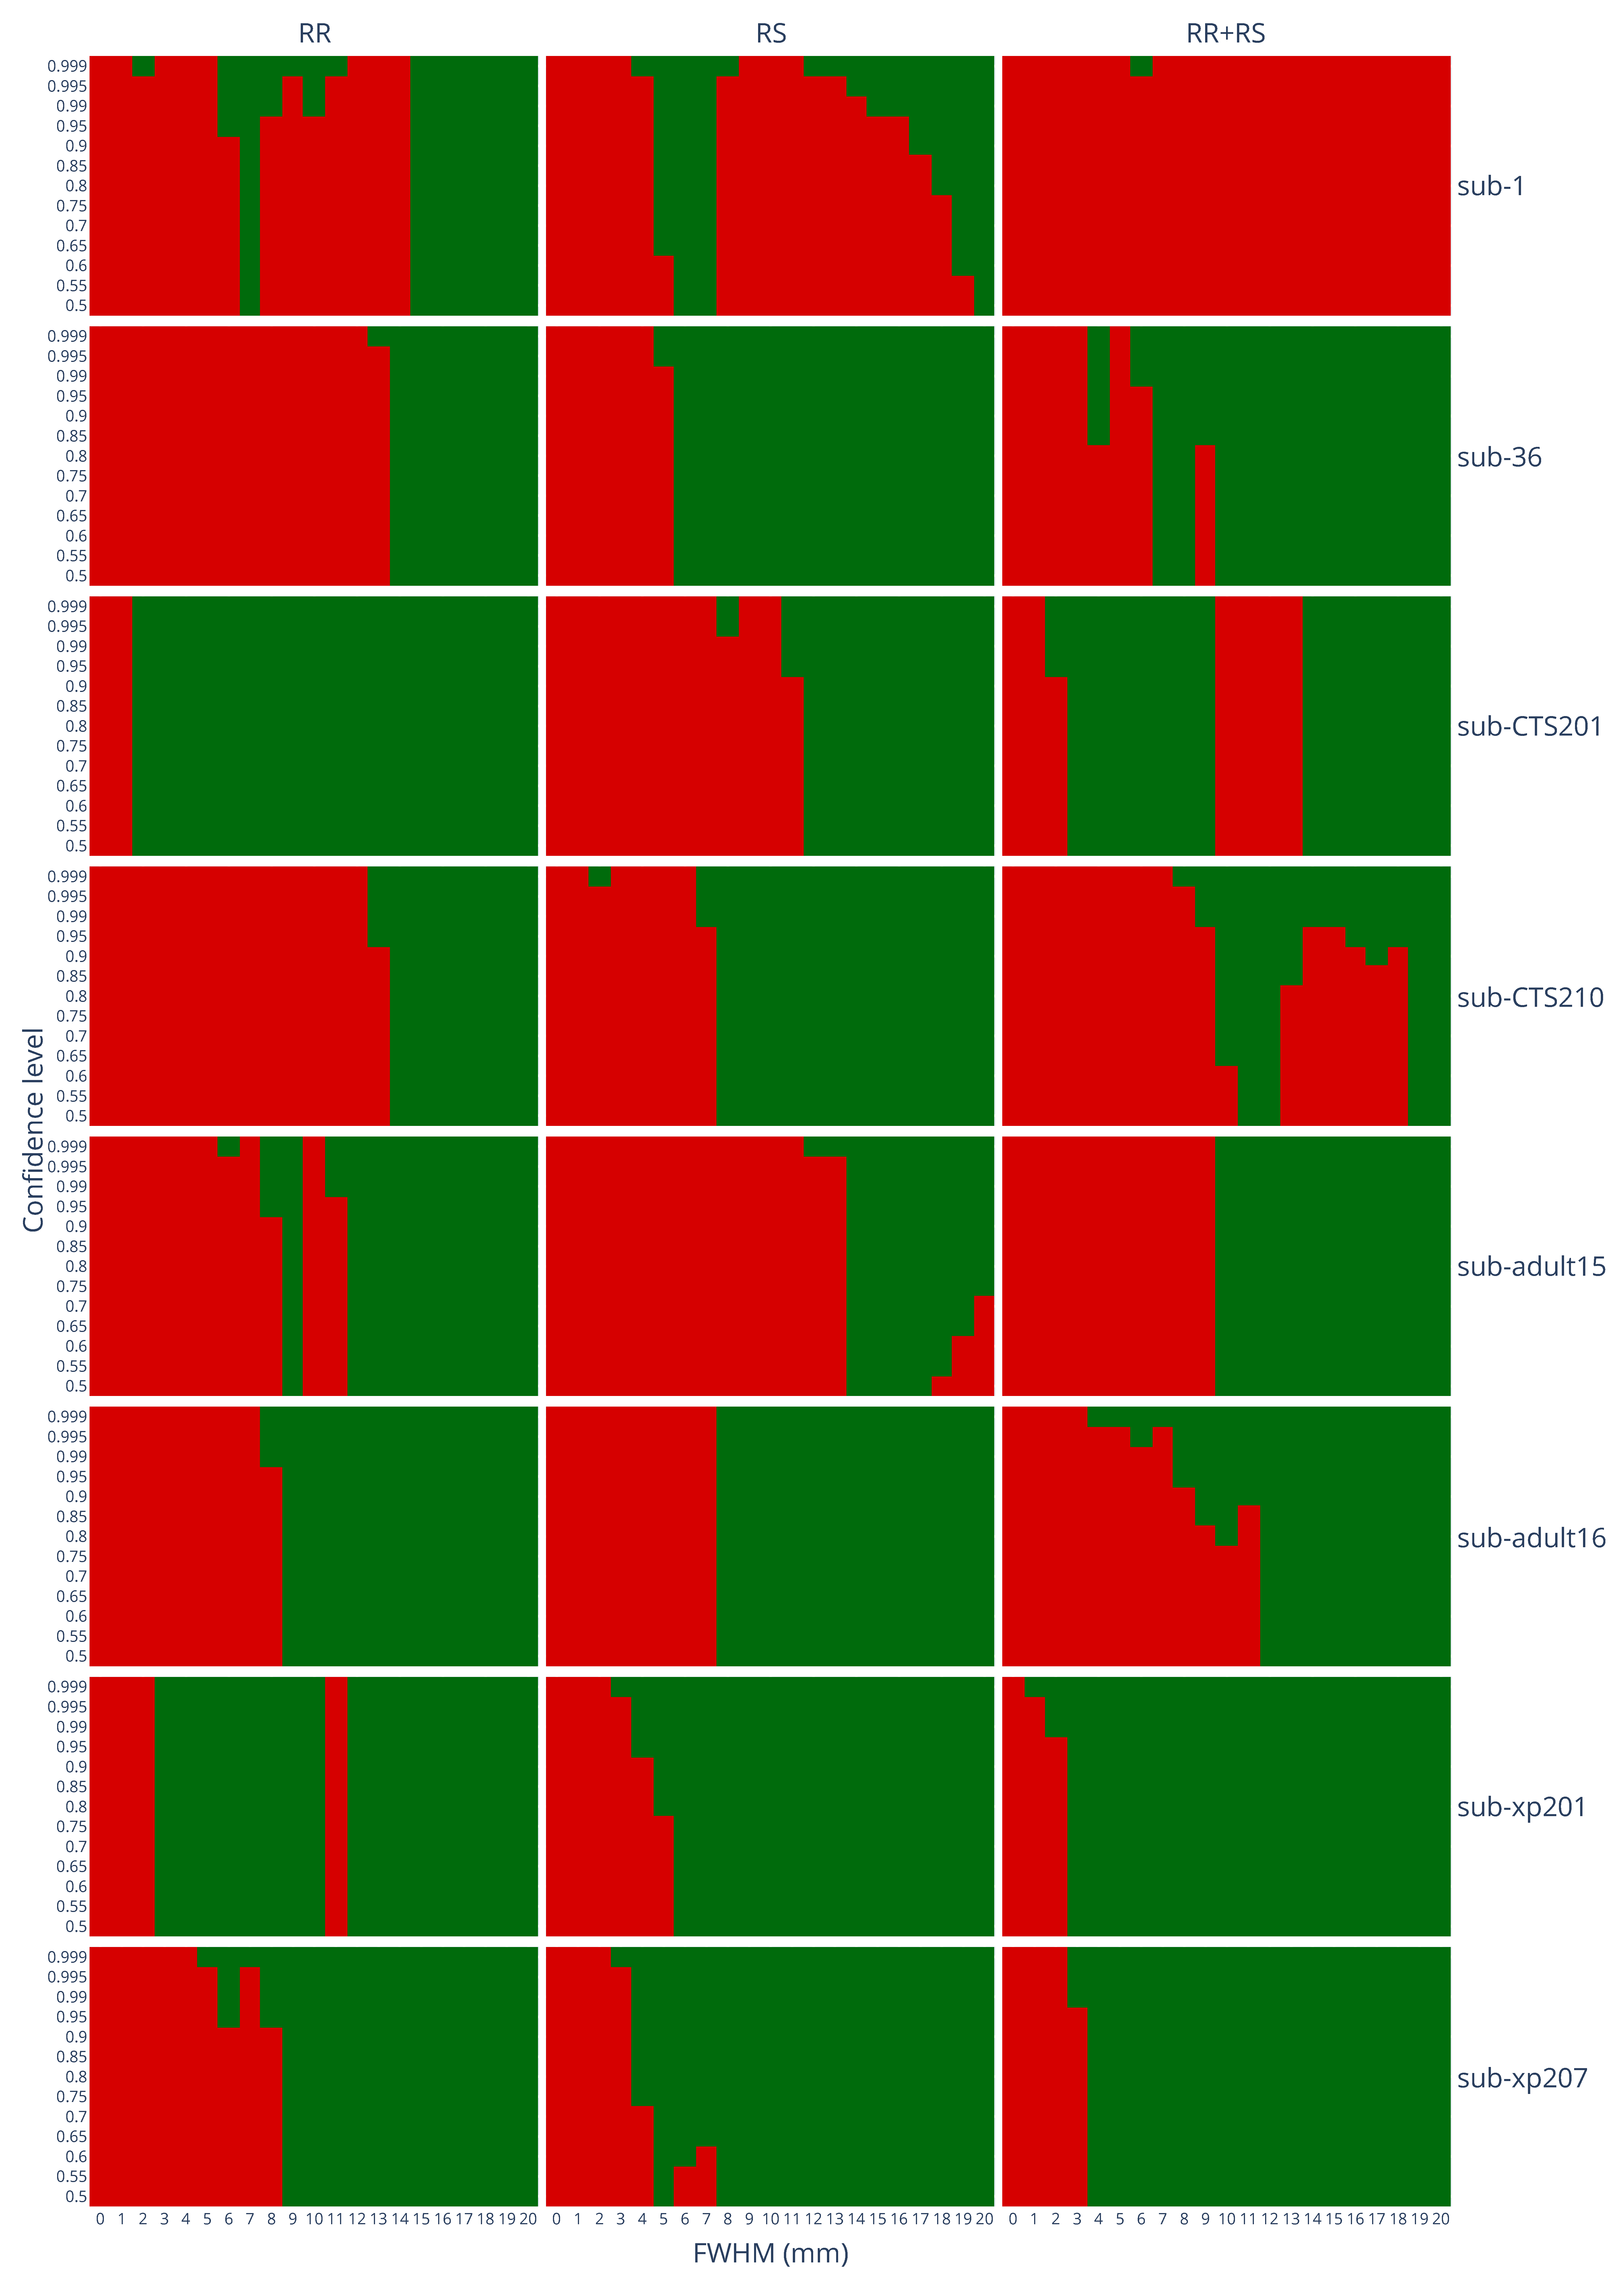
\includegraphics[width=\linewidth]{figures/ieee_mct_fwe_bonferroni.pdf}
%     \caption{IEEE check for bonferroni correction.}
% \end{figure}

% \begin{figure}
%     \centering
%     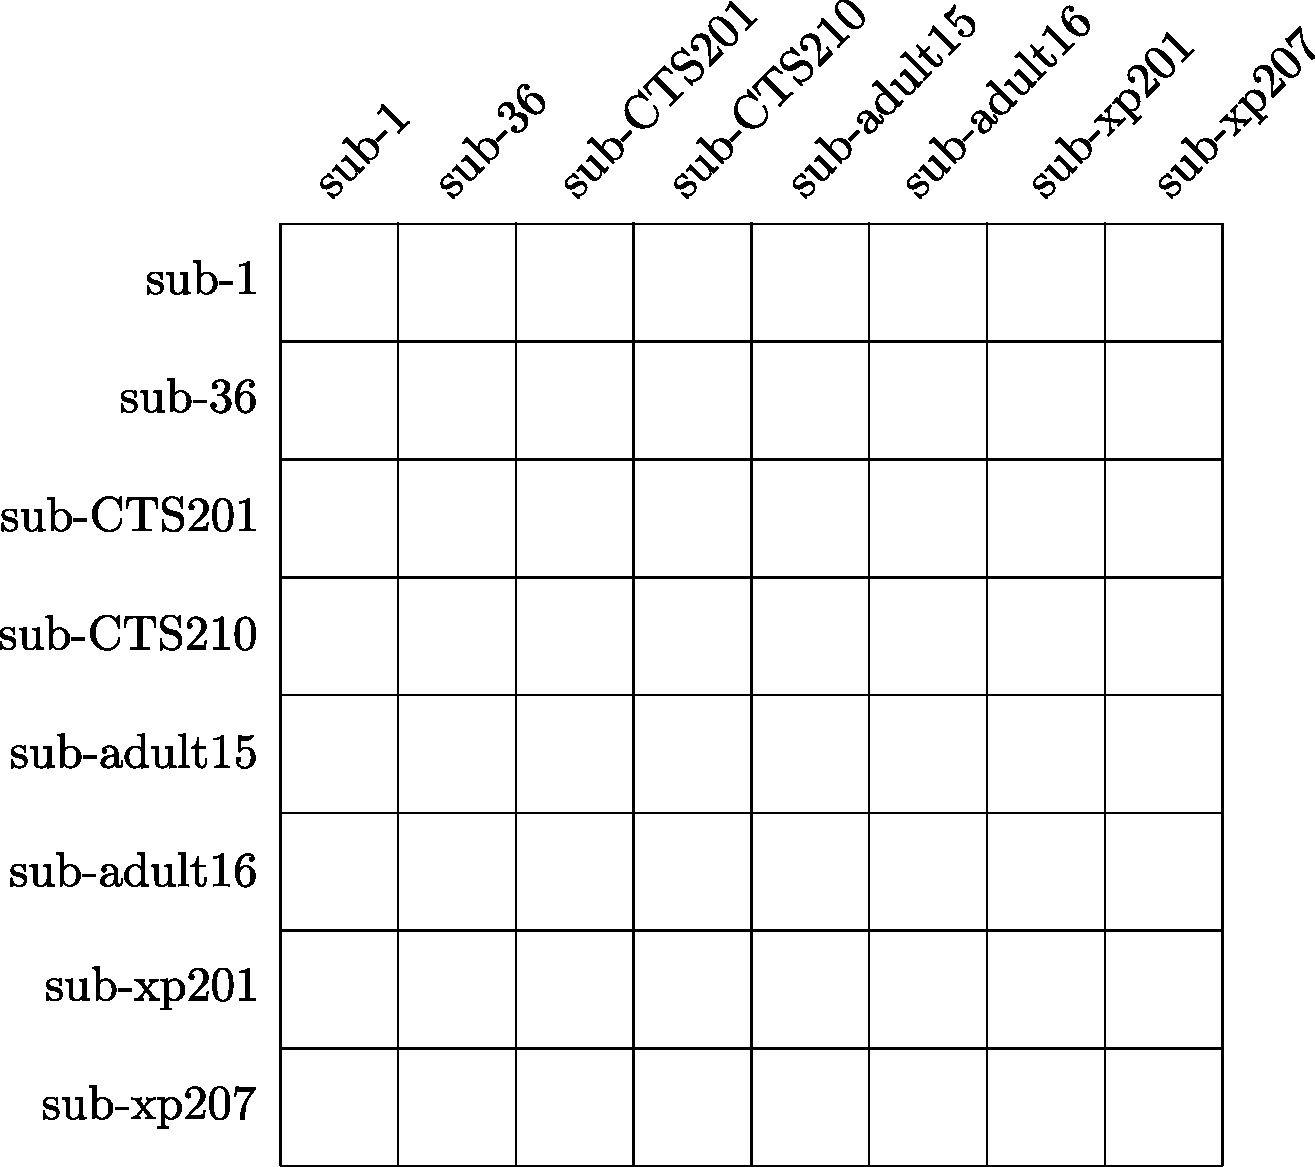
\includegraphics[width=0.3\linewidth]{figures/cross.pdf}
%     \caption{Subjects posititon in inter-subject check}
% \end{figure}



\begin{figure}
    \centering
    \begin{subfigure}[t]{0.7\linewidth}
        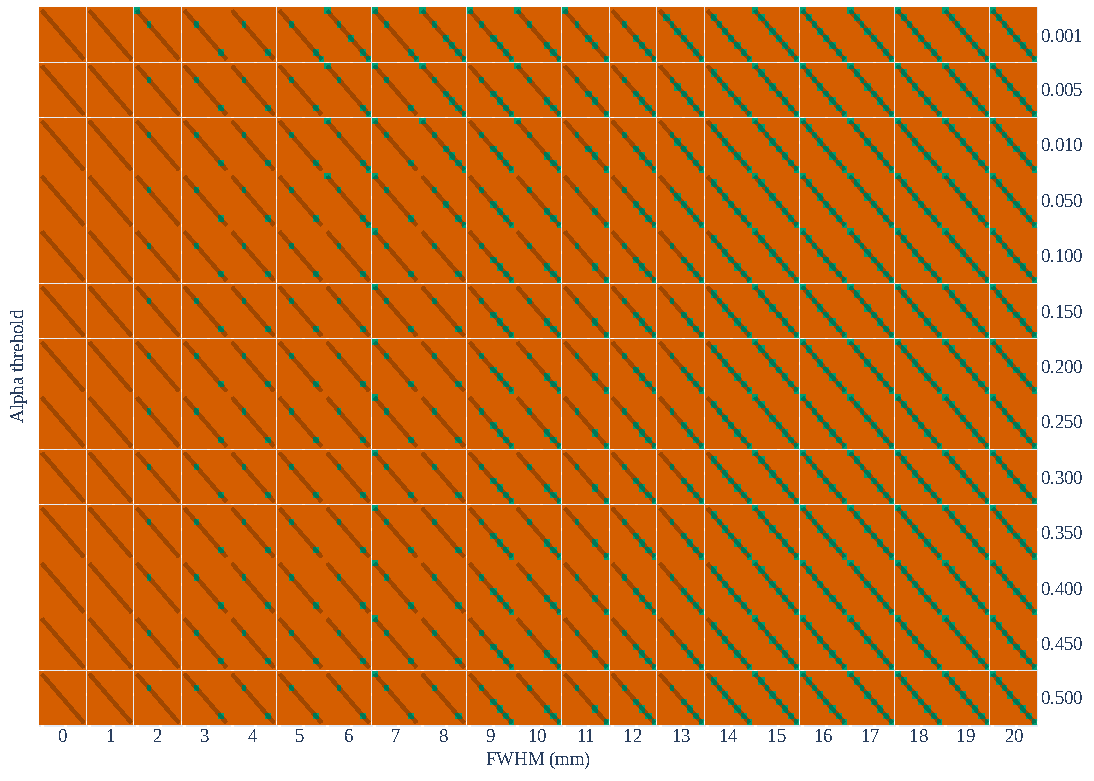
\includegraphics[width=\linewidth]{figures/inter-subject/one_mct_fwe_bonferroni_RR.pdf}
    \end{subfigure}

    \begin{subfigure}[t]{0.7\linewidth}
        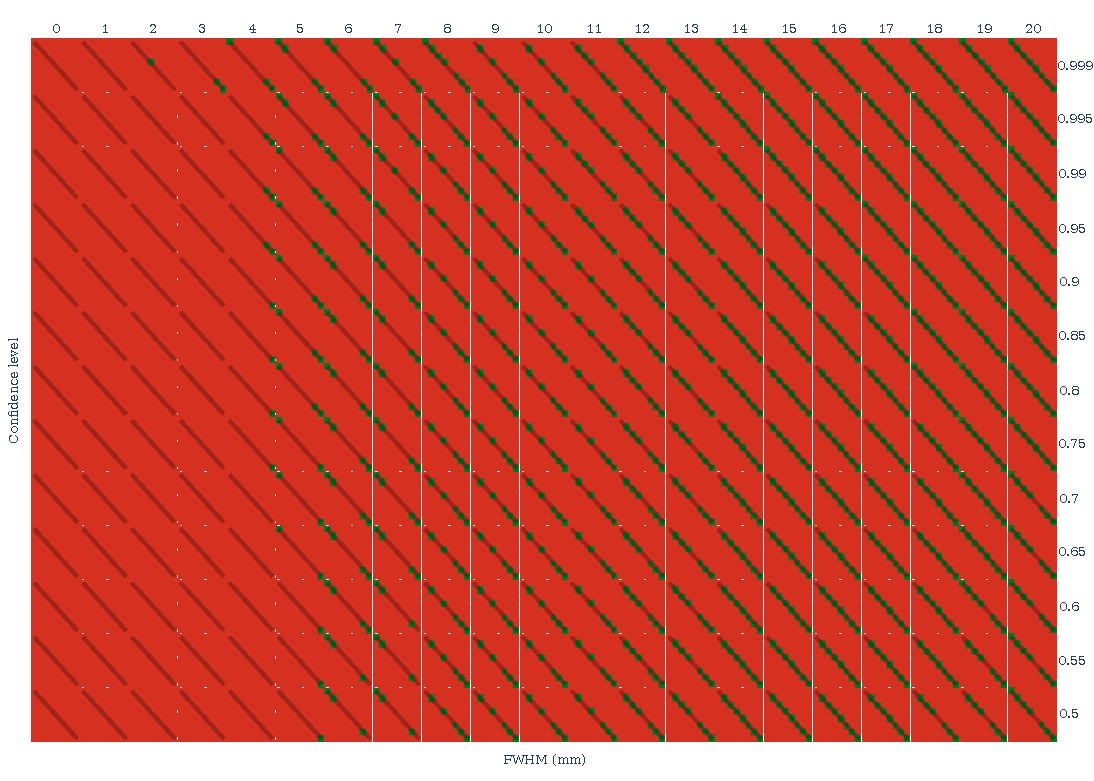
\includegraphics[width=\linewidth]{figures/inter-subject/one_mct_fwe_bonferroni_RS.pdf}
    \end{subfigure}

    \begin{subfigure}[t]{0.7\linewidth}
        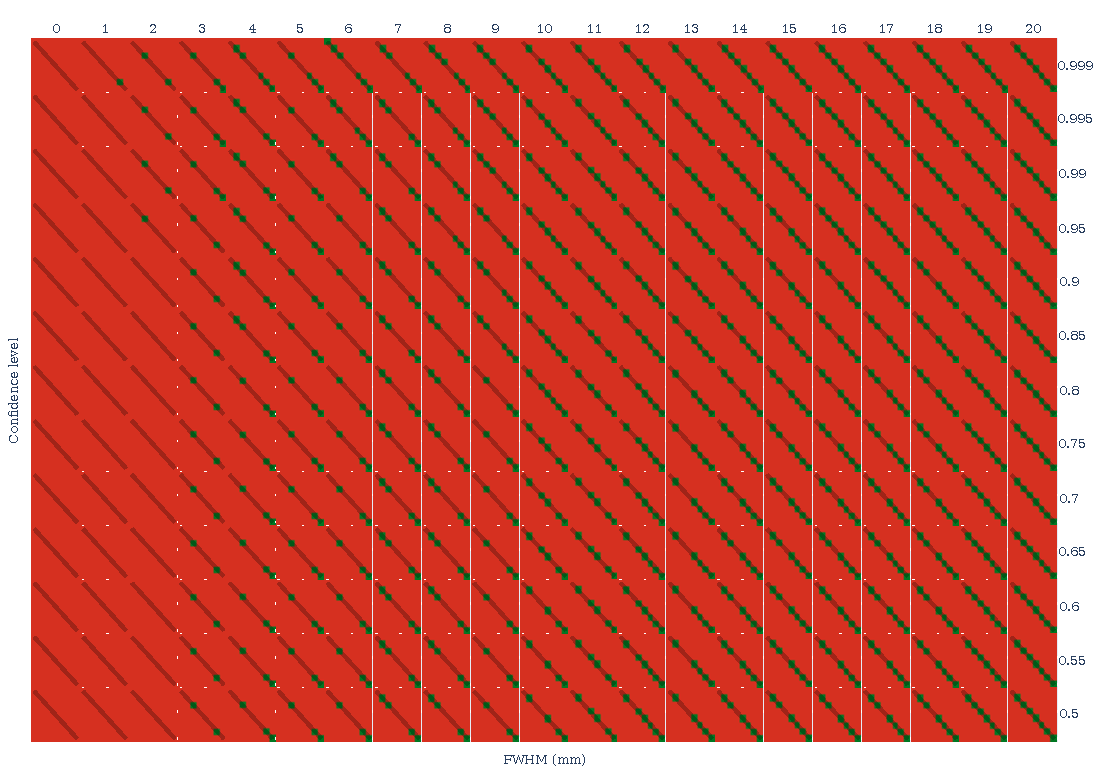
\includegraphics[width=\linewidth]{figures/inter-subject/one_mct_fwe_bonferroni_RR-RS.pdf}
    \end{subfigure}
    \label{fig:ieee-check}
    \caption{Inter-subject check for from top to bottom RR, RS and RR+RS modes (bonferroni)}
\end{figure}

\begin{figure}
    \centering
    \includegraphics[width=\linewidth]{figures/template/one_mct_fwe_bonferroni__template_annotated.pdf}
    \caption{Corrupted template check for RR, RS and RR+RS mode (bonferroni)}
\end{figure}



Conclude this section by selecting 1 test among all and use this test in the
next section.

\subsection{Non-regression test application to environment updates}

\begin{itemize}
    \item NumPy: pip upgrade numpy in existing container.
    \item Python: check if updating all or most packages works.
    \item OS: Install fmriprep in more recent Ubuntu versions. Test with Fedora
          too.
    \item Arch: narval is AMD. Check on Intel (Beluga, lab cluster).
    \item fMRIPRep: test non-LTS versions of fMRIPrep.
\end{itemize}


Then show and discuss some failed subjects.


\section{Discussion}

% summary of results
Starting from the neuroimaging use case, we have proposed an original approach
to non-regression tests in the absence of ground truth (reference) and
acceptable bounds of variation. We have applied this approach to fMRIPrep, one
of the largest processing pipeline in neuroimaging.

% conclusion
Conclusion
\begin{itemize}
    \item From a software engineering point of view, the non-regression test is usable
    ($\alpha=0.15$ and FWHM=10mm) for a well-chosen database of test subjects. Do we want 
    to build the test with a different value of alpha and FWHM for each subject?
    \item discuss sensitivity (to template corruption, subject change) vs specificity (LOO, IEEE)
\end{itemize}


This approach requires reasonable numerical stability. It also requires normal
(Gaussian) distributions of uncertainty.

On smaller examples, we could do non-parametric tests.

Discuss extension to functional pipeline.


% limitations
The Bonferroni correction assumes that all comparisons are independent, which is
not the case for brain images. The resulting test is likely to be conservative,
i.e., to not be sensitive enough to detect small deviations from the reference
distribution.

Explain that perturbations were introduced in libmath only. For other
applications (e.g., Deep Neural Networks), other libraries might have to be
perturbed.

% future work
We could do the same on different derivatives (probabilistic segmentations).


It would be interesting to investigate this approach on other use cases
including test cases as in pytracer.

\section{Conclusion}
\section{Acknowledgments}

Computations were made on the Narval supercomputer from \'Ecole de Technologie
Sup\'erieure (ETS, Montr\'eal), managed by Calcul Québec and Compute Canada. The
operation of this supercomputer is funded by the Canada Foundation for
Innovation (CFI), Ministère de l’Économie, des Sciences et de l’Innovation du
Québec (MESI) and le Fonds de recherche du Québec – Nature et technologies
(FRQ-NT).


\begin{appendices}
    \section{Results for uncorrected tests}
    \label{appendix:multiple-comparison-tests}

    In absence of multiple comparison correction, we expect
    by construction to incorrectly reject each $H_{0,i}$ with probability $\alpha$ a.k.a
    the per-comparison error rate (PCER). To account for the PCER, we measure the
    fraction of positive z-tests $V_P$ among the $v$ voxels in the image and the
    tested \fmriprep result is considered part of the reference distribution iif:
    \begin{equation}
        \label{eq:pce}
        V_{P} \leq \alpha.
    \end{equation}

    For each of the $n$ repetitions,
    we measured $V_P$, the fraction of
    positive z-tests among the $v$ voxels as well as $\mathds{1}_n$, the number of repetitions
    that passed the test with Bonferroni correction.
    
    For the uncorrected tests (Equation~\ref{eq:pce}), we expect $\overline{V_P}$ to have
    the following upper bound:
    \[
        \overline{V_P} \leq
        \alpha  + t_{29,0.05} \frac{\tilde{\sigma}_{V_P}}{\sqrt{30}}
    \]
    with
    $t_{k,\gamma}$ the $(1-\gamma)$quantile of the Student distribution with $k$ degrees of freedom,
    and $\overline{V_P}$ and $\tilde{\sigma}_{V_P}$ the mean and standard-deviation estimated from
    $n$ $V_P$ measures.
    This confidence interval is obtained from a two-tailed one-sample
    t-test with $n-1$ degrees of freedom at a level of significance $\alpha_0=0.05$:
    \[
        \mathbb{P}
        \left(
        -t_{n-1,\alpha_0/2}
        <
        \dfrac{\overline{V_p} - \alpha}{\tilde{\sigma}_{V_P} / \sqrt{n}}
        <
        t_{n-1,\alpha_0/2}
        \right)
        = 1 - \alpha_0
    \]
    
    % fraction of positive
    % z-tests $V_P$ among the $v$ voxels should be close to the nomimal value $\alpha$
    % on average. To assess the validity of our LOO test, we test that the average
    % of the $n$ $V_P$ fractions measured belongs to a confidence interval
    % around the nomimal value $\alpha$. To do so, we use  resulting in the 
    % following confidence interval for $V_P$:
    
    % obtained from:

\begin{figure}
    \centering
    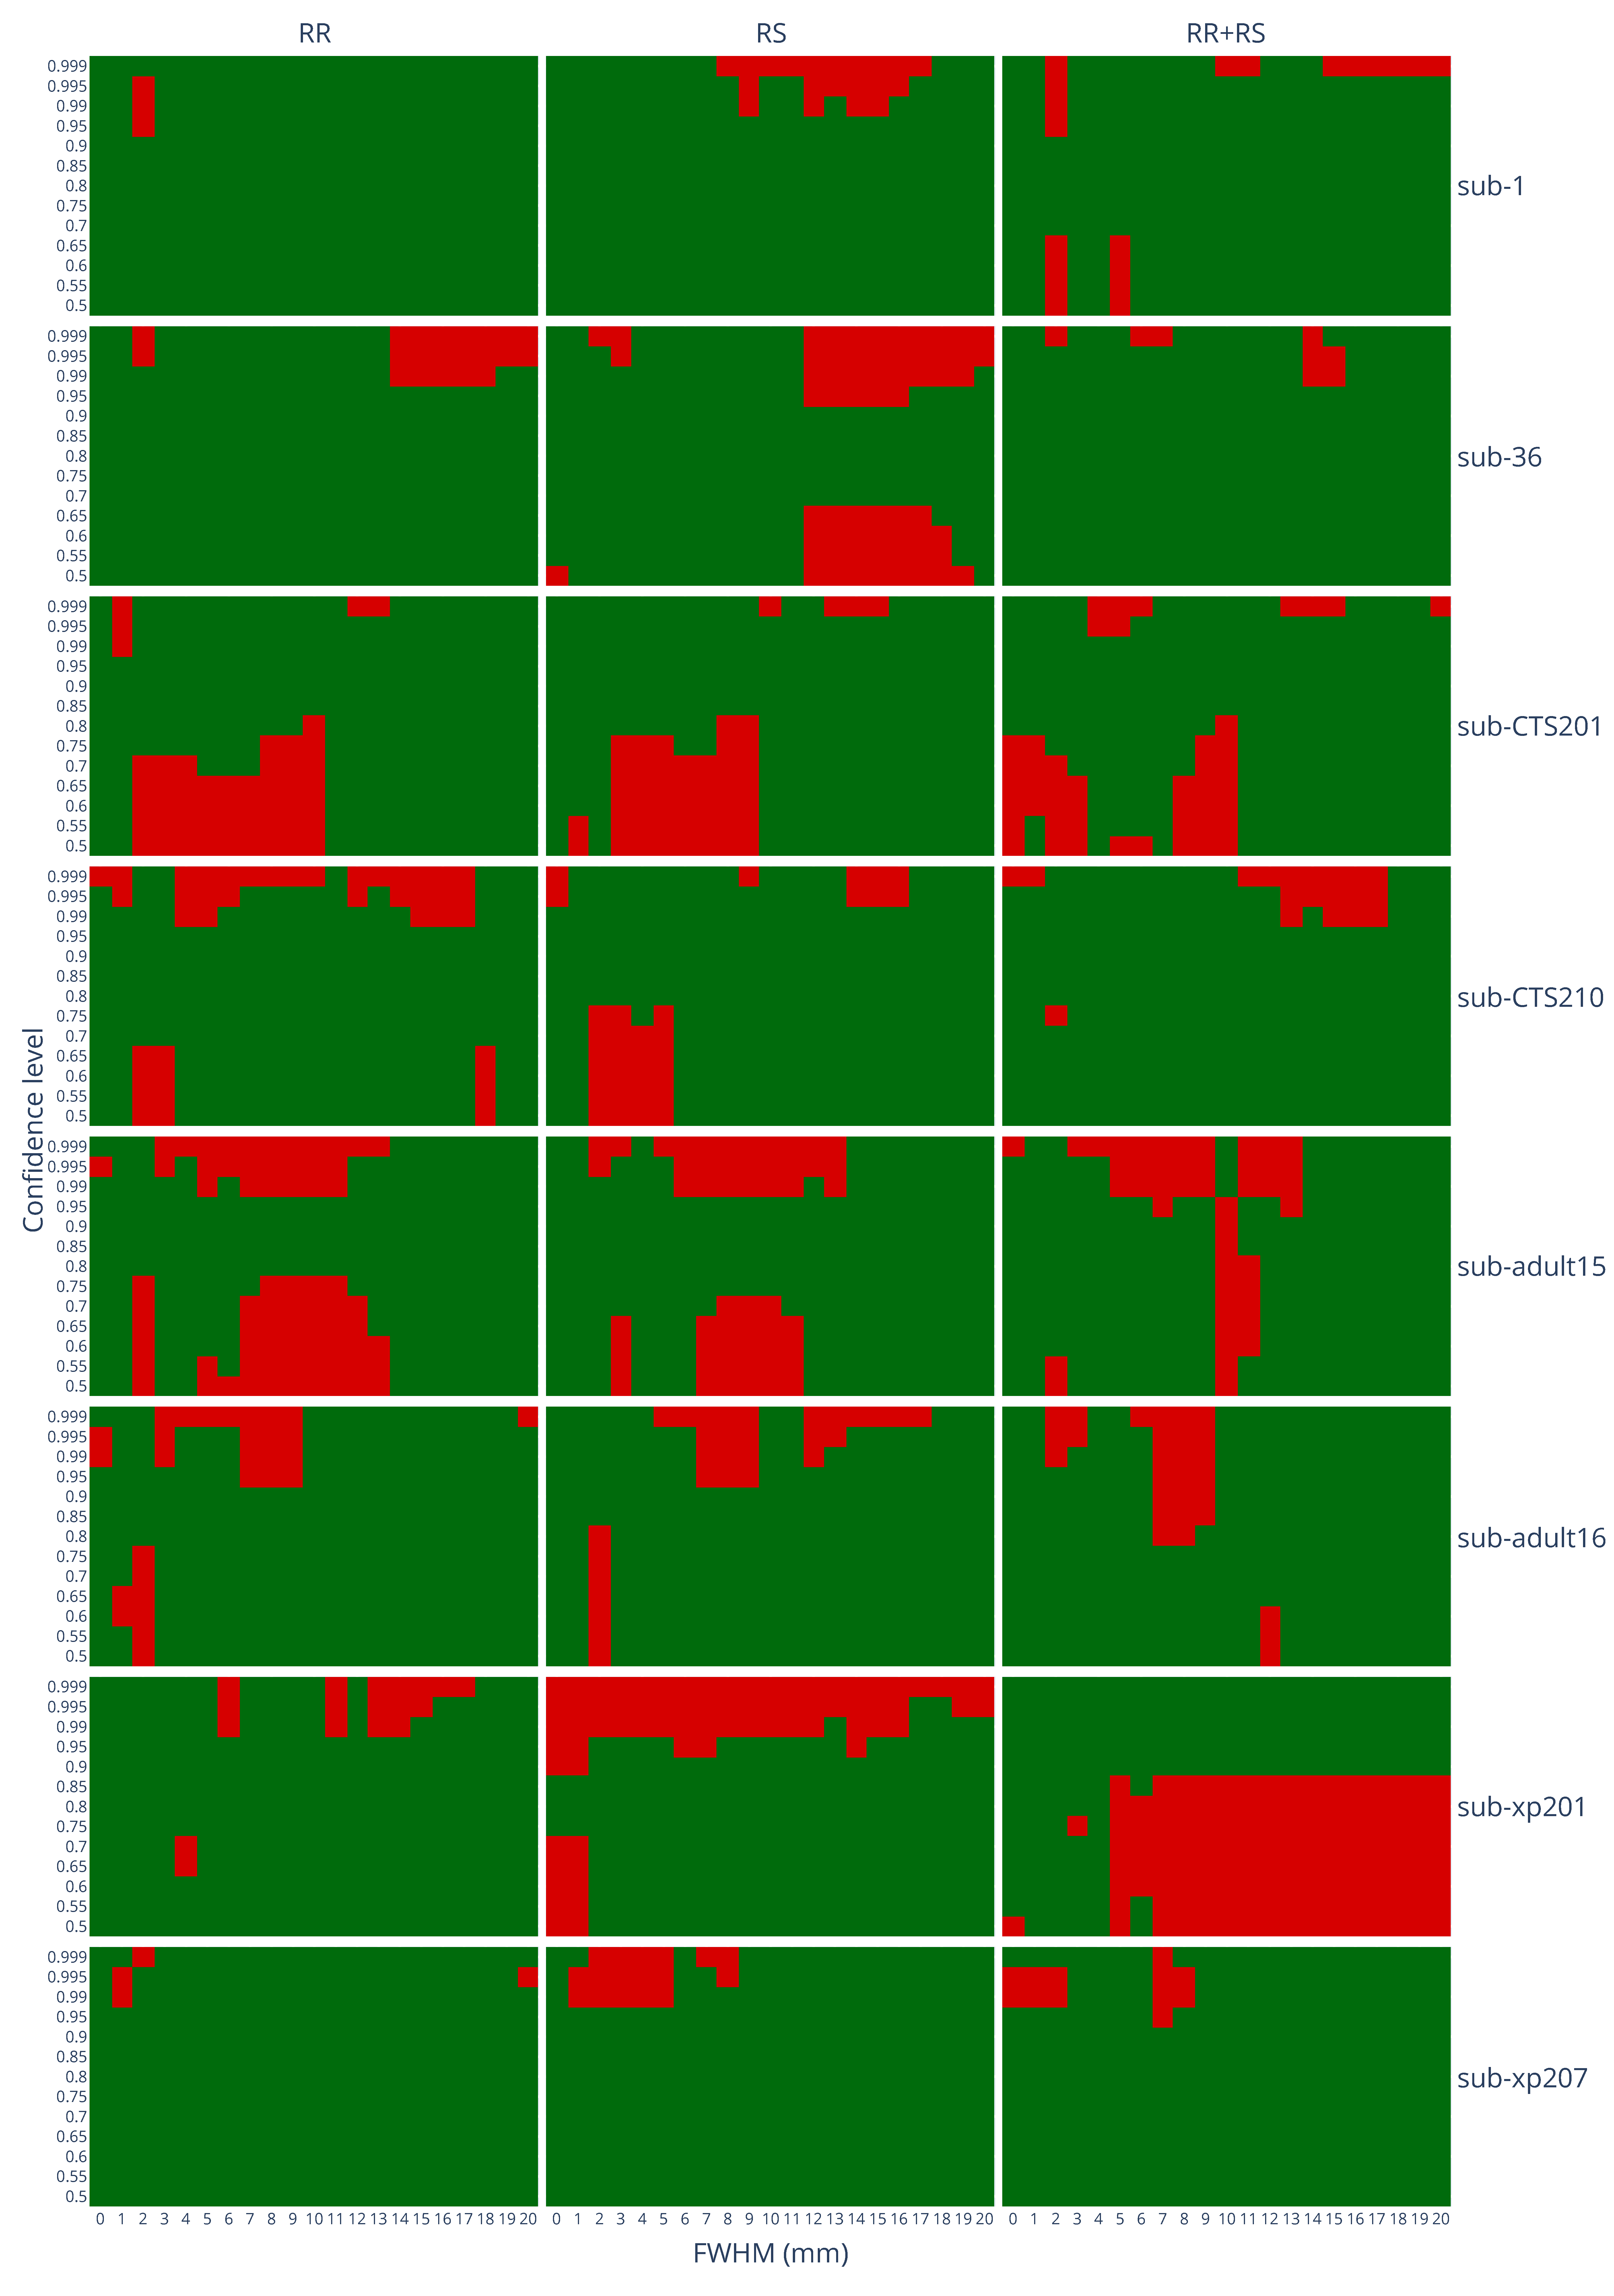
\includegraphics[width=\linewidth]{figures/exclude_pce.pdf}
    \caption{PCE}
    \label{fig:loo_pce}
\end{figure}

\begin{figure}
    \centering
    \includegraphics[width=\linewidth]{figures/template/one_pce__template_annotated.pdf}
    \caption{Corrupted template check for RR, RS and RR+RS mode (pce)}
\end{figure}

\end{appendices}


\bibliographystyle{alpha}
\bibliography{main}

\end{document}